\documentclass{../cs-classes/cs-classes}

\title{Introduction to Machine Learning}
\author{Alessandro Rudi, Umut \c{S}im\c{s}ekli\\ Notes by Antoine Groudiev}

\begin{document}
\begin{abstract}
    This document is Antoine Groudiev's class notes while following the class \emph{Introduction to Machine Learning} (Apprentissage Statistique) at the Computer Science Department of ENS Ulm. It is freely inspired by the class notes written by Pierre Gaillard, Alessandro Rudi, and Umut \c{S}im\c{s}ekli. 
\end{abstract}
\tableofcontents
\newpage

\section{An overview of Machine Learning}
%\subsection{What is ML?}
%Considering a problem, such as image classification: given an input image of a dog or a cat, the program is asked to determine whether the image is a dog or a cat. Conventional programming would hardcode the solution to this problem. But this process takes time and is not easily generalisable. Instead, an ML model is trained on a dataset to produce a program to solve the problem.
%
%Many successfull applications of Machine Learning are:
%\begin{itemize}
%    \item Face recognition
%    \item Spam filtering
%    \item Speech recognition
%    \item Self-driving systems; pedestrian detection
%\end{itemize}
%
%\subsection{Topics in Machine Learning}
%\subsubsection{Supervised Learning}
%\begin{example}[Classification]
%    Features $x\in\R^d$, labels $y\in\{1, \dots, k\}$
%\end{example}
%
%\begin{definition}[Regression]
%    Features $x\in\R^d$, labels $y\in\R$. To tackle such problem, we look for a parametrized function $f_\theta(x_i)\simeq y_i$ for some $f_\theta$ in a function space
%    \begin{equation*}
%        \mathcal{F} = \{f_\theta : \theta\in\Theta\}
%    \end{equation*}
%    Our goal is therefore to find the best function in $\mathcal{F}$ such that $f$ "fits" the training data. For example, we can say that $f$ "fits" the training data when
%    \begin{equation*}
%        \frac{1}{n}\sum_{i=1}^n (f(x_i)-y_i)^2
%    \end{equation*}
%    is "small". Such a function is not interesting in general, like for classification. 
%\end{definition}
%
%\begin{definition}[Loss function]
%    Assums that the features are in $\mathcal{X}$ and the labels are in $\mathcal{Y}$. We introduce the more general \emph{loss function} notion:
%    \begin{equation*}
%        l:\mathcal{Y}^2\to \R_+
%    \end{equation*}
%    For a regression task, we can use $l(\hat{y}, y)=(\hat{y}-y)^2$. For a classification task, $l(\hat{y}, y)=\ind_{\hat{y}=y}$.
%\end{definition}
%
%Therefore, for a regression problem, we might choose:
%\begin{equation*}
%    f^\star=\argmin_{f\in\mathcal{F}}\frac{1}{n}\sum_{i=1}^n l(f(x_i), y_i)
%\end{equation*}
%In the parametric case, when $\mathcal{F}=\{f_\theta : \theta\in\Theta\}$, we might minimize with respect to $\theta$:
%\begin{equation*}
%    \theta^\star=\argmin_{\theta\in\Theta}\frac{1}{n}\sum_{i=1}^n l(f(x_i), y_i)
%\end{equation*}
%
%\subsubsection{Probabilistic approach}
%Let $\mathcal{Z}=\mathcal{X}\times\mathcal{Y}$ be the feature space. Let $D$ be a distribution on $\mathcal{Z}$; we make the assumption that the training data is iid from $D$:
%\begin{equation*}
%    (x_i, y_i)\sim D
%\end{equation*}
%and the same thing hold for the test data:
%\begin{equation*}
%    (\tilde{x_i}, \tilde{y_i})\sim D
%\end{equation*}
%According to the Strong Law of Large Numbers, the test loss converges almost surely:
%\begin{equation*}
%    \lim_{n\to\infty}\frac{1}{n}\sum_{i=1}^n l(f_\theta(\tilde{x_i}), \tilde{y_i}) = \E_{(x, y)\sim D}[l(f_\theta(x), y)] =: R(\theta)=R(f_\theta)
%\end{equation*}
%where $R(\theta)$ is the \emph{population risk}.
%
%\begin{definition}[Risk minimization]
%    
%\end{definition}
%
%\subsubsection{Unsupervised Learning}
%\begin{example}[Clustering]
%    
%\end{example}
%
%\begin{example}[Dimensionnality reduction]
%    We are given features $x\in \R^d$ and labels $y\in\{0, 1\}$ which form a "training" dataset $S=\{(x_1, y_1), \dots, (x_n, y_n)\}$. We assume that $d\gg1$; our goal is to find $d'\ll d$ such that $(x_1, y_1, \dots, )$
%\end{example}

\section{Linear Least Squares Regression}
%Consider an input space $X$ and an output space $Y$. We consider a function $f:X\to Y$ unknown to us, that we want to recover. We are given samples $D_N = [(x_1, y_1), \dots, (x_N, y_N)]$. Our goal is to produce $\hatf_D$ such that $\hatf_D$ "converges" to $f$ when $|D|\to+\infty$.
\subsection{Introduction}
In this chapter, we will study the simple but still widely used problem of \emph{Linear Least Square Regression}. We are given a set of points, which we assume to be sampled from some distribution: there exists some function which generated these points, and we want to retrieve or at least approximate this unknown function. To do so, we will naturally look for the function which best fits the points; nevertheless, assuming that it is unlikely that the function is overly-complicated, we will only approximate it using \emph{linear function}. Finally, to choose which linear function \say{fits best} the data, we will introduce the mean square error, which we will minimize to find our linear approximation function.

Formally, our objective is to find a function $f$ such that it explains well the distribution $(y_i)_{1\leq i\leq n}$ as a function of $(x_i)_{1\leq i\leq n}$, that is $y_i\sim f(x_i)$. To do this, we can choose a \emph{function space} $\mathcal{F}$ and solve the empirical risk minimization problem:
\begin{equation*}
    \hatf_n \in \argmin_{f\in\mathcal{F}} \hat{R}_n(f) := \argmin_{f\in\mathcal{F}} \frac{1}{n}\sum_{i=1}^n (y_i-f(x_i))^2
\end{equation*}
\begin{wrapfigure}[12]{l}{0.34\textwidth}
    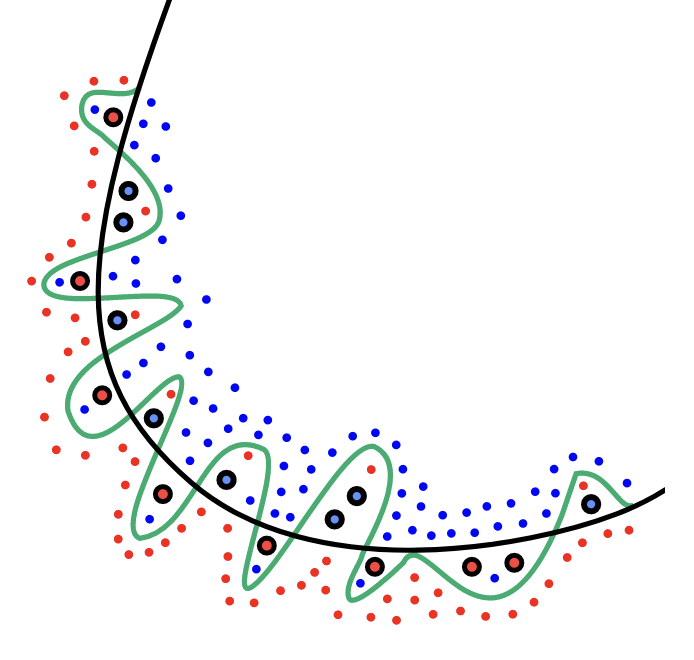
\includegraphics[width=0.3\textwidth]{images/overfitting.png}
    \caption{Example of overfitting}
\end{wrapfigure}

Care must be taken when selecting the function space to avoid overfitting\footnote{We say that the function \emph{overfits} the data when it corresponds too closely to the specific set of data (i.e.~on the training data), such that it fails to fit additional data (i.e.~test data).}: for example, if we were to choose $\mathcal{F}:=\R_d[X]$ for some $d\in\N$, it is in our best interest to keep $d$ small to avoid getting a function $f$ which fits perfectly the points but diverges between them. Although the empirical mean square error $\hat{R}_n$ decreases when the function space $\mathcal{F}$ becomes larger (i.e.~larger polynomial degrees), the $\hatf_n$ estimator loses its predictive power. $\hatf_n$ will not necessarily perform well on new data. In what follows, we will consider the linear function space, containing functions of the form $f:x\mapsto ax+b$, which is the simplest.

\subsection{General setup and notations for supervised learning}
\begin{definition}[Training data set]
    The \emph{training data set}, often denoted $D_n:=\set{(x_i, y_i)}{i\in\llbracket 1, n \rrbracket}$, is the set of some observations $(x_i, y_i)\in\X\times\Y$. We will often make the assumption that the observations $(x_i, y_i)$ are realizations of i.i.d. random variables from a distribution $\nu$.
\end{definition}

The distribution $\nu$ is unknown to the statistician; it's a matter of learning it from the data.

\begin{definition}[Learning rule]
    A \emph{learning rule} $\A$ is a function that associates to training data $D_n$ a prediction function $\hatf_n$:
    \begin{equation*}
        \begin{aligned}
            \A: \bigcup_{n\in\N} (\X\times\Y)^n &\longrightarrow \Y^\X\\
            D_n &\longmapsto \hatf_n
        \end{aligned}
    \end{equation*}
    The estimated function $\hatf_n$ is constructed to predict a new output $y$ from a new input $x$, where $(x, y)$ is a pair of \emph{test data}, i.e.~not necessarily observed in the training data. The function $\hatf_n$ is an estimator because it depends on the data $D_n$ and not on unobserved parameter, such as the distribution $\nu$. If $D_n$ is random, it is also a random function.
\end{definition}

\begin{definition}[Squared Loss Risk]
    Given an estimator $\hatf_n$, we define its risk:
    \begin{equation}
        \label{eq:sq-risk}
        \risk(\hatf_n) := \E\left[(Y-\hatf_n(X))^2\,\big| \, D_n\right] \quad \textnormal{where} \quad (X, Y)\sim\nu
    \end{equation}
    This is also called the \emph{generalization error}, as it measures how well the estimator performs on other inputs and outputs of the dataset.
\end{definition}

In practice, the statistician cannot compute the risk, since one cannot acces the distribution $\nu$. Therefore, a common method in supervised machine learning is to replace the risk (defined using the distribution $\nu$ through the expectation $\E$) by the empirical risk (defined using the training data set).

\begin{definition}[Squared Loss Empirical risk]
    Given an estimator $\hatf_n$ and a data set $D_n=\set{(x_i, y_i)}{i\in\iset{1}{n}}$, we define its \emph{empirical risk}:
    \begin{equation}
        \label{eq:sq-empirical-risk}
        \emrisk_n(\hatf_n) := \frac{1}{n}\sum_{i=1}^n (y_i-\hatf_n(x_i))^2
    \end{equation}
\end{definition}

\begin{wrapfigure}[15]{r}{0.45\textwidth}
    \centering
    \captionsetup{justification=centering}
    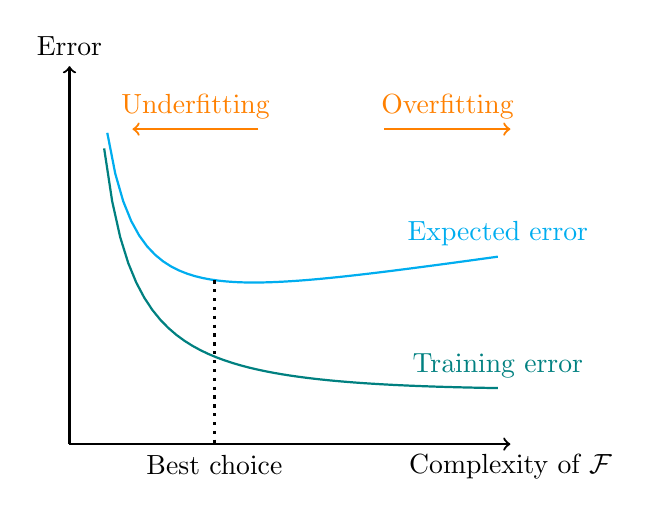
\begin{tikzpicture}[scale=0.8]
        \draw[domain=0.55:6.8, samples=50, color=teal, thick] plot (\x, 2.5/\x + 0.2*\x^0.5) node[above] {Training error};
        \draw[domain=0.6:6.8, samples=50, color=cyan, thick] plot (\x, 2.5/\x + 1*\x^0.5) node[above] {Expected error};
        \draw[dotted, very thick] (2.3, 2.6) -- (2.3, 0) node[below] {Best choice};
        \draw[->, thick] (0,0) -- (7,0) node[below] {Complexity of $\mathcal{F}$};
        \draw[->, thick] (0,0) -- (0,6) node[above] {Error};

        \draw[->, color=orange, thick] (5, 5) -- (7, 5) node[above, pos=0.5] {Overfitting};
        \draw[->, color=orange, thick] (3, 5) -- (1, 5) node[above, pos=0.5] {Underfitting};
      \end{tikzpicture}
    \caption{Overfitting and underfitting}
\end{wrapfigure}
However, one must be careful about overfitting, the case where $\emrisk_n(f)$ is much lower than $\risk(f)$, as discussed previously. In this chapter, we will study the performance of the least square estimator in the case of the linear model.

\begin{definition}[Linear model]
    When $\X=\R^d$ and $\Y=\R$, the simplest interesting function space is the set of affine functions. To ease the notation, we assume that the frist components of the inputs is 1 so that it is sufficient to consider linear functions. Therefore, the function space is:
    \begin{equation}
        \mathcal{F}:=\set{x\mapsto \theta^\tp x}{\theta\in\R^d}
    \end{equation}
    i.e.~linear functions parametrized by $\theta\in\R^d$.
\end{definition}

\begin{remark}
    Choosing a linear model, the empirical risk minimization corresponds to the problem of minimizing the following quantity over $\theta\in\R^d$:
    \begin{equation*}
        \emrisk_n(\theta):=\frac{1}{n}\sum_{i=1}^n(y_i-\theta^\tp x_i)^2
    \end{equation*}
    This expression can be rewritten using matrix notation. We let $Y=(Y_1, \dots, Y_n)^\tp\in\R^n$ be the vector of outputs and $X\in\R^{n\times d}$ the matrix of inputs, whose rows are $x_i^\tp$. $X$ is called the \emph{design matrix}. The empirical risk is therefore given by:
    \begin{equation*}
        \emrisk_n(\theta)=\frac{1}{n}\norm{Y-X\theta}^2_2
    \end{equation*}
\end{remark}

\subsection{Ordinary Least Squares Estimator (OLS)}
\subsubsection{Definition and closed form}
In the following, we assume that the design matrix is injective.\footnote{Said otherwise, the rank of $X$ is $d$.} In particular, $d\leq n$, otherwise this is not possible.

\begin{definition}[Ordinary Least Squares]
    If $X$ is injective, the minimizer of the empirical risk \eqref{eq:sq-empirical-risk} is called the \emph{Ordinary Least Squares (OLS) estimator}. Said otherwise, it is the vector $\htheta\in\R^d$ minimizing $\emrisk_n$:
    \begin{equation}
        \label{eq:ols-estimator}
        \htheta := \argmin_{\theta\in\R^d} \emrisk_n(\theta)=\argmin_{\theta\in\R^d}\frac{1}{n}\sum_{i=1}^n(y_i-\theta^\tp x_i)^2
    \end{equation}
\end{definition}

\begin{property}[Closed form soluion of the OLS estimator]
    \label{prop:closed-form-OLS}
    If $X$ is injective, the OLS estimator exists and is unique. Moreover, it is given by:
    \begin{equation}
        \label{eq:closed-form-OLS}
        \htheta = (X^\tp X)^{-1}X^\tp Y
    \end{equation}
\end{property}

\begin{proof}
    Since $\emrisk_n$ is coercive\footnote{$\norm{\emrisk_n(\theta)} \xrightarrow[\norm{\theta}\to+\infty]{} +\infty$} and continuous, it admits at least a minimizer. Furthermore, we have:
    \begin{equation*}
        \emrisk_n(\theta) := \frac{1}{n}\norm{Y-X\theta}^2_2 = \frac{1}{n}\left(\theta^\tp(X^\tp X)\theta - 2\theta^\tp X^\theta Y+\norm{Y}^2\right)
    \end{equation*}
    Since $\emrisk$ is differentialble any mimizer cancels its gradient:
    \begin{equation*}
        \nabla\emrisk_n(\htheta) = \frac{1}{n}\left(\htheta^\tp(X^\tp X) + (X^\tp X)\htheta - 2X^\tp Y\right) = \frac{2}{n}\left((X^\tp X)\htheta - Y^\tp X\right)
    \end{equation*}
    where the last equality holds because $X^\tp X\in\R^{d\times d}$ is symmetric. Since $X$ is injective, $X^\tp X$ is invertible\footnote{It is even positive definite.}. Therefore, a solution of $\nabla\emrisk_n(\htheta)=0$ satisfies:
    \begin{equation*}
        \htheta = (X^\tp X)^{-1}XY
    \end{equation*}
    Finally, this unique solution is indeed a minimum since its Hessian is definite positive:
    \begin{equation*}
        \nabla^2\emrisk_n(\htheta) = \frac{2}{n}(X^\tp X)
    \end{equation*}
\end{proof}

\subsubsection{Geometric interpretation}
The linear model aims modeling the ouput vector $Y\in\R^n$ by a linear combination of the form $X\theta\in\R^n$. The image of $X$ is the solution space, denoted:
\begin{equation*}
    \im(X)=\set{X\theta\in\R^n}{\theta\in\R^d}
\end{equation*}
This is the vector subspace of $\R^n$ generated by the $d\leq n$ columns of the design matrix. As $\rg(X)=d$, it is of dimension $d$.

By minimizing $\norm{Y-X\theta}$, we thus look for the element of $\im(X)$ closest to $Y$. This is the orthogonal projection of $Y$ on $\im(X)$, denoted $\hat{Y}$. By definition of the OLS and by Property \ref{prop:closed-form-OLS}, we have:
\begin{equation*}
    \hat{Y} := X\htheta = X(X^\tp X)^{-1}X^\tp Y
\end{equation*}
In particular, $P_X:=X(X^\tp X)^{-1}X^\tp$ is the projection matrix on $\im(X)$.

\subsubsection{Numerical resolution}
The closed form formula \eqref{eq:closed-form-OLS} of the OLS is useful in analyzing it; however, calculating it naively can be prohibitively expensive. For example, when $d$ is large, one prefers to avoid inverting the design matrix $X^\tp X$ which costs $O(d^3)$\footnote{Using the Gauss-Jordan method}, and can be very unstable when the matrix is badly conditioned. The following methods are usually preferred.

\paragraph*{QR factorization}
To improve stability, $QR$ decomposition can be used. Since $\htheta$ is the solution of the equation:
\begin{equation*}
    (X^\tp X)\htheta = X^\tp Y
\end{equation*}
we write $X\in\R^{n\times d}$ as $X=QR$ where $Q\in\R^{n\times d}$ is an orthogonal matrix\footnote{That is $QQ^\tp=I_n$} and $R\in\R^{d\times d}$ is upper triangular. Upper triangular matrices are very useful for solving linear systems. Substituting in the previous equation, we get:
\begin{equation*}
    \begin{aligned}
        R^\tp(Q^\tp Q)R\htheta = R^\tp Q^\tp Y &\iff R^\tp R\htheta = R^\tp Q^\tp Y \\
        &\impliedby R\htheta = Q^\tp Y
    \end{aligned}
\end{equation*}
All that remains is to solve a linear system with a triangular upper matrix, which is easy.

\begin{wrapfigure}[11]{l}{0.5\textwidth}
    \centering
    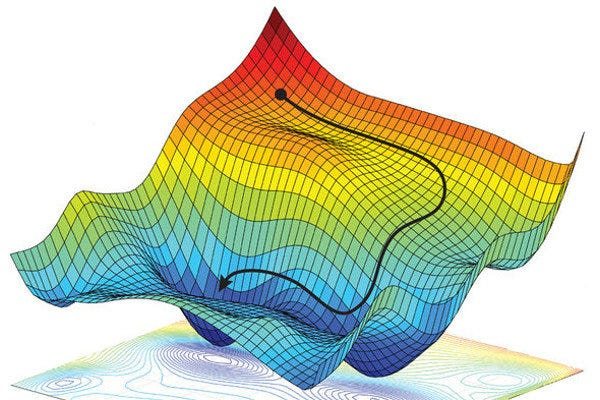
\includegraphics[width=0.4\textwidth]{images/gradient-descent.jpg}
    \caption{(Non-convex) Gradient descent}
\end{wrapfigure}
\paragraph*{Gradient descent}
We can completely bypass the need of matrix inversion or factorization using gradient descent. It consists in solving the minimization problem step by step by approching the minimum throught gradient steps. For example, we initialize $\theta_0:=0$\footnote{In practice, $\theta_0$ is often initialized to some random vector to avoid singularities.}, then update it using the following recurrence formula:
\begin{equation*}
    \begin{aligned}
        \theta_{i+1} :=&\, \theta_i -\eta\cdot\nabla\emrisk_n(\theta_i)\\
        =&\, \theta_i - \eta\cdot\frac{2}{n}\left((X^\tp X)\theta_i - Y^\tp X\right)
    \end{aligned}
\end{equation*}
where $\eta>0$ is a learning parameter called \emph{learning rate}. We see that if the algorithm converges, then it converges to a point cancelling the gradient, thus to the (unique) OLS solution. For the algorithm to converge, the learning rate $\eta$ must be well calibrated. This will be seen in more details in the following chapter about gradient descent.

If the data set is too big, i.e.~when $n\gg1$, loading all the data to make the gradient calculation $\nabla\emrisk(\theta_i)$ can be prohibitively expensive too. The common solution to this is to use \emph{Stochastic Gradient Descent}, where gradient calculations for one step are made only on estimates of $\nabla\emrisk(\theta_i)$, calculated on a random subset of the data.

\subsubsection{Nonlinear problem: polynomial, spline, and kernel regression}
The assumption tha the observations $y_i$ can be explained as a linear combination of the explanatory variables $x_{i, j}$ may seem strong. However, the previous linear framework can be applied to transformations of the variables $x_{i, j}$. For example, by adding the powers of the variables $x^k_{i, j}$ or their products $x_{i, j}\cdot x_{i', j'}$, this allows comparison to polynomial spaces. Doing a linear regression on polynomial transformations of variables is equivalent to doing a polynomial regression.

Of course, other bases and transformations exist: for instance, \emph{spline bases} are piecewise polynomials with constraints on the edgets. This is the model used for example by EDF to predict electricity consumption as a function of variables such as the time of the day, the day of the week, temperature or cloud cover.
In general, we can consider transformations $\varphi:\X\to\R^d$ and try to explain the outputs $y_i$ with functions of the form $\theta\to\varphi(x_i)^\tp \theta$. Another form of regression that we will discuss in the following is therefore \emph{kernel regression}, which allows computing efficiently the estimator even when $\varphi$ maps to an infinite dimensional space.

\subsection{Statistical analysis}
In this section, we try to show some guarantees for the OLS estimator, such as a bound the excess risk of the OLS, which we will define later on.
\subsubsection{Stochastic assumptions and bias/variance decomposition}
To provide guarantees on the performance of OLS, we require assumptions about how the data is generated. In this section, we consider a stochastic framework that will allow us to statistically analyze OLS.

\paragraph*{Assumption: linear model}
We assume that there exists a vector $\theta^*\in\R^d$ such that for all $1\leq i\leq n$, 
\begin{equation}
    \label{eq:assumption-linear-model}
    Y_i = x_i^\tp \theta^* + Z_i
\end{equation}
where $Z=(Z_1, \dots, Z_n)^\tp\in\R^n$ is a vector of \emph{errors}, also called \emph{noise}. The $Z_i$ are assumed to be centered independent variables of variance $\sigma^2$, i.e. $\E[Z_i]=0$ and $\V[Z_i]=\sigma^2$. The assumption \eqref{eq:assumption-linear-model} can be rewritten in matrix form:
\begin{equation}
    Y=X\theta^*+Z
\end{equation}
where $Y=(Y_1, \dots, Y_n)^\tp\in\R^n$, $X=(x_1, \dots, x_n)^\tp\in\R^{n\times d}$, and $Z=(Z_1, \dots, Z_n)^\tp\in\R^n$.

\begin{remark}
    We write $Y_i$ and $Z_i$ using capital letters to remind ourselves that they are random variables. The noise $Z$ comes from the fact that in practice, the observations $Y_i$ never completely fit the linear forecast. They are due to noise or unobserved explanatory variables. As before, we assume that the first vector of the explanatory variable is the constant vector, i.e. $\forall i, x_{i, 1}=1$
\end{remark}

\paragraph*{Analysis settings}
Two settings of analysis can be chosen:
\begin{itemize}
    \item In the \emph{fixed desing} setting, the design matrix $X$ is not random but deterministic and the features $x_1, \dots, x_n$ are fixed. The expectations are thus only with respect to the $Z_i$ and the $Y_i$, and the goal is to minimize:
    \begin{equation*}
        \risk_X(\theta) = \E\left[\frac{1}{n}\sum_{i=1}^n (Y_i-x_i^\tp\theta)^2\right]
    \end{equation*}
    for new random observations $Y_i$, but on the same inputs.
    \item In the \emph{random design} setting, both the inputs and the ouputs are random. This is the most standard setting in supervised machine learning. The goal is therefore to minimize the risk \eqref{eq:sq-risk} -- also called the generalization error.
\end{itemize}
In this chapter, we will consider the fixed design setting, because it eases both the notation and the calculations -- we will only need some simple linear algebra.

Before analyzing the statistical properties of OLS, we state a general result under the linear model assumption, which illustrates the tradeoff between estimation and approximation -- or bias and variance.

\begin{property}[Risk decomposition]
    Under the linear model assumption with fixed design, the following hols:
    \begin{equation*}
        \forall \theta\in\R^d, \quad \E[\risk_X(\theta)-\risk_X(\theta^*)] = \norm{\theta-\theta^*}^2_\Sigma
    \end{equation*}
    where $\Sigma:=\frac{1}{n}X^\tp X\in\R^{d\times d}$ and $\norm{\alpha}^2_\Sigma:=\alpha^\tp\Sigma\alpha$. Furthermore, if $\theta$ is a random variable -- when it depends on a random dataset -- we have:
    \begin{equation*}
        \E[\risk_X(\theta)]-\risk(\theta^*) = \underbrace{\norm{\E[\theta]-\theta^*}^2_\Sigma}_{\textnormal{Bias}} + \underbrace{\E\left[\norm{\theta-\E[\theta]}^2_\Sigma\right]}_{\textnormal{Variance}}
    \end{equation*}
\end{property}
\begin{proof}
    %TODO
\end{proof}

\begin{remark}
    It is worth to note that the optimal risk satisfies:
    \begin{equation*}
        \risk_X(\theta^*) = \E\left[\frac{1}{n}\sum_{i=1}^n(Y_i-x_i^\top\theta^*)^2\right] = \E\left[\frac{1}{n}\sum_{i=1}^nZ_i^2\right] = \frac{1}{n}\sum_{i=1}^n\E[Z_i^2]=\sigma^2
    \end{equation*}
\end{remark}

\subsubsection{Statistical properties of OLS}
We can now show some guarantees for the OLS estimator.

\begin{property}
    Under the linear model assumption with fixed design, the OLS estimator $\htheta$ defined by \eqref{eq:ols-estimator} satisfies:
    \begin{equation*}
        \E[\htheta] = \theta^* \quad \textnormal{and} \quad \V[\htheta] = \frac{\sigma^2}{n}\Sigma^{-1}
    \end{equation*}
    i.e. it is unbiased, and its variance is some $O(n^{-1})$. Furthermore, we can even show that it satisfies the Gauss-Markov property: it is optimal among all unbiased estimators of $\theta$, in the sense that is has a minimal variance-covariance matrix.
\end{property}

\begin{proof}
    %TODO
\end{proof}

\begin{definition}[Excess risk]
    The excess risk of an estimator $\htheta$ is defined by:
    \begin{equation}
        \E[R_X(\htheta)]-\risk(\theta^*)
    \end{equation}
    It allows to measure the risk induced by the use of an estimator instead of the optimal vector, without taking into account the inherent risk generated by the noise, which cannot be reduced.
\end{definition}

\begin{corollary}[Excess risk of OLS]
    Under the linear model assumption with fixed design, the excess risk of the OLS satisfies:
    \begin{equation*}
        \E[\risk_X(\htheta)]-\risk(\theta^*)=\frac{\sigma^2d}{n}
    \end{equation*}
\end{corollary}

\begin{proof}
    % TODO
\end{proof}

\subsubsection{Gaussian noise model}
A special case that is often considered is Gaussian noise, i.e. $Z_i\sim\mathcal{N}(0, \sigma^2)$, the normal distribution of expectation 0 and variance $\sigma^2$. This choice comes not only from the fact that it allows to compute many additional statistical properties on $\htheta$ and to perform tests, such as confidence intervals or significance of variables. In practice, it is also motivated by the central limit theorem, and the fact that noise is often an addition of many phonomena not explained by the linear combination of the explanatory variables.

\begin{property}
    In the linear model with Gaussian noise, the maximum likelihood estimators of $\theta$ and $\sigma$ satisfy respectively:
    \begin{equation*}
        \htheta_{MV}=(X^\tp X)^{-1}XY \quad \textnormal{and} \quad \hat{\sigma}^2_{MV}=\frac{\norm{Y-X\htheta}^2}{n}
    \end{equation*}
    We therefore find the least squares estimator obtained by minimizing the empirical risk. The variance estimator is biased. We will see more about maximum likelihood estimators in next chapters.
\end{property}

\subsection{Ridge regression}
\subsubsection{Handling non-injective design matrices}
If $X$ is not injective, the matrix $X^\tp X$ is no longer invertible and the OLS optimization problem admits several solutions. The problem is said to be \emph{poorly posed} or \emph{unindentifiable}. Since the variance of $\htheta$ depends on the conditioning of the matrix $(X^\tp X)^{-1}$, the more columns of it are likely to be dependent, the less stable $\htheta$ will be. Several solutions allow dealing with the case where $\rg(X)<D$.

\emph{Explicit complexity control} reduces the $\im(X)$ solution space: this can be done by removing columns from the $X$ matrix until it becomes injective (for example, by reducing the degree of polynomials). One can also set identifiability constraints of the form $\theta\in V$, a vector subspace of $\R^d$ such that any element $y\in\im(X)$ has a unique antecedent $\theta\in V$ with $y=X\theta$. For example, we could choose $V=\ker(X)^\bot$.

\emph{Implicit complexity control} regularizes the empirical risk minimization problem. The most common approach is to regularize by adding $\norm{\theta}^2_2$ (Ridge regression) or $\norm{\theta}_1$ (Lasso regression).

\subsubsection{Ridge regression}
\begin{definition}
    For a regularization parameter $\lambda$, the Ridge regression estimator is defined as
    \begin{equation}
        \htheta_\lambda \in \argmin\set{\frac{1}{n}\norm{Y-X\theta}^2_2+\lambda\norm{\theta}^2_2}{\theta\in\R^d}
    \end{equation}
    The regularization parameter $\lambda>0$ regulates the trade-off between the variance of $\htheta$ and its bias.
\end{definition}

\begin{property}
    The Ridge regression estimator is unique and satisfies:
    \begin{equation*}
        \htheta_\lambda = (X^\tp X+n\lambda I_n)^{-1}X^\tp Y
    \end{equation*}
\end{property}
\begin{proof}
    Similar to the one of the OLS and left as an exercise. We can see that there is no longer the problem of inverting $X\tp X$ since the Ridge regression replaces $(X^\tp X)^{-1}$ by $(X^\tp X+n\lambda I_n)^{-1}$ in the OLS solution.
\end{proof}

\begin{property}[Risk of Ridge regression]
    Under the linear model assumption, the Ridge regression estimator satisfies:
    \begin{equation*}
        \E[\risk_X(\htheta_\lambda)]-\risk_X(\theta^*) = \sum_{j=1}^d(\theta_j^*)^2\frac{\lambda_j}{(1+\lambda_j/\lambda)^2} + \frac{\sigma^2}{n}\sum_{j=1}^d\frac{\lambda_j^2}{(\lambda_j+\lambda)^2}
    \end{equation*}
    where $\lambda_j$ is the $j$-th eigenvalue of $\Sigma=\frac{1}{n}X^\tp X$. In particular, the choice of:
    \begin{equation*}
        \lambda^* = \frac{\sigma\sqrt{\Tr(\Sigma)}}{\norm{\theta^*}_2\sqrt{n}}
    \end{equation*}
    yiels the following excess risk:
    \begin{equation*}
        \E[\risk_X(\htheta_{\lambda^*})]-\risk_X(\theta^*) \leq \frac{\sigma\sqrt{2\Tr(\Sigma)\norm{\theta^*}_2}}{\sqrt{n}}
    \end{equation*}
\end{property}
\begin{proof}
    Follows from the bias-variance decomposition, and is left as an exercise.
\end{proof}

\begin{remark}
    As $\lambda\to0$, its excess risk converges to the one of OLS. The first term corresponds to the bias of the Ridge estimator. Thus, on the downside, the Ridge estimator is biased in constrast to the OLS. But on the positive side, its variance does not involve the inverse of $\Sigma$ but of $\Sigma+\lambda I_d$ instead, which is better conditioned. It has therefore a lower variance. The parameter $\lambda$ controls the trade-off.
\end{remark}

\subsubsection{Comparaison to the OLS}
We can compare the excess risk bound obtained by $\htheta_{\lambda^*}$ with the one of the OLS, which was $\sigma^2d/n$.
\begin{itemize}
    \item The OLS convergence is in $O(n^{-1})$ while the convergence of $O(n^{-1/2})$, which is slower
    \item The OLS dependency on the noise is in $\sigma^2$ while Ridge's is in $\sigma$, which is better
    \item Since $\Tr(\Sigma)\leq\max_{1\leq i\leq n}\norm{x_i}^2$, if the input norms are bounded by $R$, the excess risk of Ridge does not depend on the dimension $d$, which can even be infinite. It is called a \emph{dimension free} bound.
\end{itemize}
The calibration of the regularization parameter is therefore essential in practice. It can for example be done analytically as in the proposition -- but often, some quantities such as $\sigma^2$ and $\norm{\theta^*}$ are unknown. In practice, one resorts to train/validation set or \emph{cross-validation}.

\section{Logistic regression and convex analysis}
%\subsection*{Recap of important notions and notations}
%We are given an input space $X$ and an output space $Y$. We want to learn the relationship between input and output, modelised by a probability distribution $\rho\in \P(X\times Y)$. Thus, we try to find the best function $f_\star:X\to Y$, given a loss function $l:Y\times Y\to\R$. Therefore, $f_\star$ is often defined by:
%\begin{equation*}
%    f_\star = \argmin_{f:X\to Y} \E_{X, Y}[l(f(X), Y)]
%\end{equation*}
%where
%\begin{equation*}
%    \E_{X, Y}[g(X, Y)] = \int_{\R^2} g(x, y) \cdot \mathrm{d}\rho(x, y)
%\end{equation*}
%
%In practice, you only know some samples $D_N=[(x_1, y_1), \dots, (x_N, y_N)]$ with $(x_i, y_i) \sim \rho$, making it impossible to choose such an $f_\star$. Therefore, we try to find a good model $\hatf_{D_N}$, such that
%\begin{equation*}
%    \lim_{N\to+\infty}\mathcal{E}(\hatf_{D_N}) - \mathcal{E}(f) = 0
%\end{equation*}
%Such a result will often be given by a \emph{learning rate function} $c(N)$, with
%\begin{equation*}
%    \E_{D_N}[\mathcal{E}(\hatf_{D_N}) - \mathcal{E}(f)] \leq c(N) = o(1)
%\end{equation*}
%The function $\hatf_{D_N}$ can be chosen such that it minimizes the empirical error:
%\begin{equation*}
%    \hatf_{D_N} = \argmin_{f\in\mathcal{H}}\hat{\mathcal{E}}(f) = \argmin_{f\in\mathcal{H}} \frac{1}{N} \sum_{i=1}^N l(f(x_i), y_i)
%\end{equation*}
%
%\subsection{}
%We consider the case where $X=\R^d$ and $Y=\R$. We define the loss $l$ to be the least squares, $l(y, y') = (y-y')^2$, and we choose our functions to be of the form of $f_\star = \theta_\star^T X$. In this case, ERM is OLS:
%\begin{equation*}
%    \htheta_N = \argmin_{\theta\in\R^d} \frac{1}{N} \sum_{i=1}^N (\theta^Tx_i-y_i)^2
%\end{equation*}
%
%We can also define $\htheta_{N, \lambda}$ to be:
%\begin{equation*}
%    \htheta_{N, \lambda} = \argmin_{\theta\in\R^d} \frac{1}{N} \sum_{i=1}^N (\theta^Tx_i-y_i)^2 + \lambda\norm{\theta}^2
%\end{equation*}
%This allows to regulate the "complexity" of the function to avoid overfitting. This is called Tikhonov regularization. In this case, we have
%\begin{equation*}
%    \E_{\hat{Y}}[\mathcal{\htheta_N} - \mathcal{E}(\theta_\star)] = \frac{\sigma^2 d}{N}
%\end{equation*}
%and therefore the optimal function is 
%\begin{equation*}
%    \hatf_{N, \lambda} = \argmin_{f\in\mathcal{H}} \hat{\mathcal{E}}(f) + \lambda R(f)
%\end{equation*}
%
%We define $X\in\R^{N\times d} := (x_1^T, \dots, x_N^T)$, and $\hat{Y}=(\hat{y}_1, \dots, \hat{y}_n)$. We this notation, we have
%\begin{equation*}
%    \htheta_{N, \lambda} = \frac{1}{N}||X\theta-\hat{Y}||^2 + \lambda||\theta||^2
%\end{equation*}
%Thus, we have
%\begin{equation*}
%    \begin{aligned}
%        \nabla\mathcal{L}(\theta) := \frac{2}{N}X^TX\theta - 2\frac{X^T\hat{Y}}{N}+2\lambda\theta &= 0\\
%        (\frac{X^TX}{N}+\lambda)\theta &= X^T\hat{Y}
%    \end{aligned}
%\end{equation*}
%therefore,
%\begin{equation*}
%    \htheta_{N, \lambda} = \left(\frac{X^TX}{N}+\lambda I\right)^{-1}\frac{X^T\hat{Y}}{N} = \left(X^TX+\lambda N I\right)^{-1}X^T\hat{Y}
%\end{equation*}
%We introduce the singular value decomposition of $X$:
%\begin{equation*}
%    X = U\Sigma V^T
%\end{equation*}
%where $U^TU = UU^T = I_N$, $V^TV = VV^T=I_d$, and $\Sigma$ is diagonal with $\forall i, \,\Sigma_{i, i} \geq 0$.
%In this case,
%\begin{equation*}
%\begin{aligned}
%    X^TX + \lambda NI_d &= V\Sigma U^T U \Sigma V^T + \lambda N I_d\\
%    &= V(\underbrace{\Sigma^2 + \lambda N I}_{\textnormal{invertible}}) V^T
%\end{aligned}
%\end{equation*}

This chapter will introduce logistic regression, a widely used classification algorithm. Unlike linear regression, there is no closed-form solution and one needs to solve it using iterative convex optimization algorithms.

\subsection{Logistic regression}
We consider the binary classification problem: given inputs in $\R^d$, we want to predict outputs in $\{0, 1\}$. We are given a training set $D_n=\set{(X_i, Y_i)}{i\in\iset{1}{n}}$, where the data points $(X_i, Y_i)$ are i.i.d. random variables following a distribution $\nu$ in $\X\times\Y=\R^d\times\{0, 1\}$

\subsubsection{Motivation}
We would like to use an algorithm similar to linear regression introduced in the previous chapter. However, since the outputs $Y_i$ are binary and belong to $\{0, 1\}$, a discrete set, we cannot predict them using a linear transformation of the inputs $X_i$. We will thus classify the data based on a classification rule of the form
\begin{equation*}
    f : \R^d \longrightarrow \R
\end{equation*}
which will then be passed through a function with specification $\R\to\{0, 1\}$. The final estimator will therefore be:
\begin{equation*}
    \ind_{\R_+}\circ f
\end{equation*}
meaning that the estimator will predict $Y_i=+1$ exactly when $f(X_i)\geq0$.

More precisely, we will consider linear functions $f$ of the form:
\begin{equation*}
    f_\beta = x \longmapsto x^\tp\beta
\end{equation*}
This assumes that the data is \emph{linearly separable}, meaning that it can be well-explained by a linear separation.
\begin{figure}[H]
    \centering
    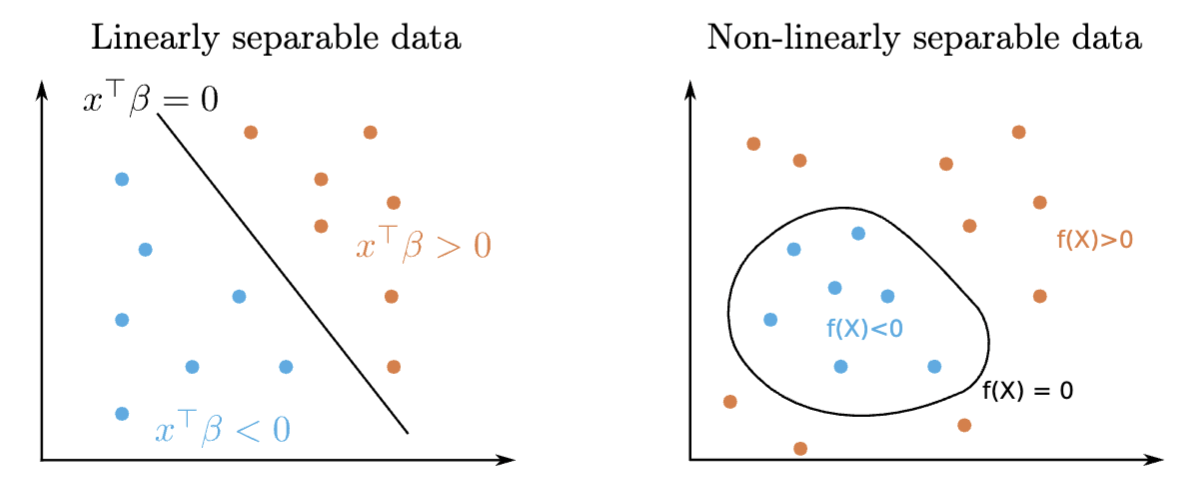
\includegraphics[width=0.8\textwidth]{images/linearly-separable.png}
    \caption{Data that can or cannot be well-explained by a linear separation}
\end{figure}
If the data does not seem to be linearly separable, we can use similar tricks as the one introduced for linear regression (polynomial regression, kernel regression, splines, \dots). We will dive into more details in an upcoming chapter about kernels.

\subsubsection{Loss function}
To minimize the empirical risk, it remains to choose a loss function to assess the performance of a prediction. 

\begin{definition}[Loss function]
    A \emph{loss function} $\ell$ is a function of the form
    \begin{equation*}
        \ell : \Y\times\Y' \longrightarrow \R_+
    \end{equation*}
    such that for $(y, y')\in\Y\times\Y'$, $\ell(y, y')$ intuitively quantifies the mistake when predicting $y'$ instead of $y$. 
\end{definition}

\begin{definition}[Empirical Risk associated to a Loss function]
    Given an estimator $\hatf_n$, a data set $D_n=\set{(x_i, y_i)}{i\in\iset{1}{n}}$ and a loss function $\ell$, we define the \emph{empirical risk associated to $\ell$} by:
    \begin{equation}
        \label{eq:em-risk-loss-function}
        \emrisk_n(\hatf_n) := \frac{1}{n}\sum_{i=1}^n \ell(y_i, \hatf_n(x_i))
    \end{equation}
\end{definition}

\begin{definition}[Squared loss]
    We define the \emph{squared loss} $\ell_2:\R\times\R\to\R_+$ used previously in linear regression by:
    \begin{equation}
        \ell_2(y, y') := (y-y')^2
    \end{equation}
    Using the squared loss $\ell_2$ in \eqref{eq:em-risk-loss-function}, we obtain the same result as the original definition \eqref{eq:sq-empirical-risk}. 
\end{definition}

\begin{definition}[Binary loss]
    A natural loss is the \emph{binary loss}, also known as the \emph{0-1 loss}. It takes 1 as a value if there is a mistake (i.e. $f(X_i)\neq Y_i$) and 0 otherwise:
    \begin{equation}
        \ell_{1}(X_i, Y_i) = \delta_{Y_i\neq\ind_{\R_+}(f(X_i))}
    \end{equation}
    Using $\ell_1$, the empirical risk becomes:
    \begin{equation*}
        \emrisk_n(\beta) = \frac{1}{n}\sum_{i=1}^n \delta_{Y_i\neq\ind_{\R_+}(X_i^\tp\beta)}
    \end{equation*}
\end{definition}

\begin{wrapfigure}{r}{0.45\textwidth}
\centering
    \captionsetup{justification=centering}
    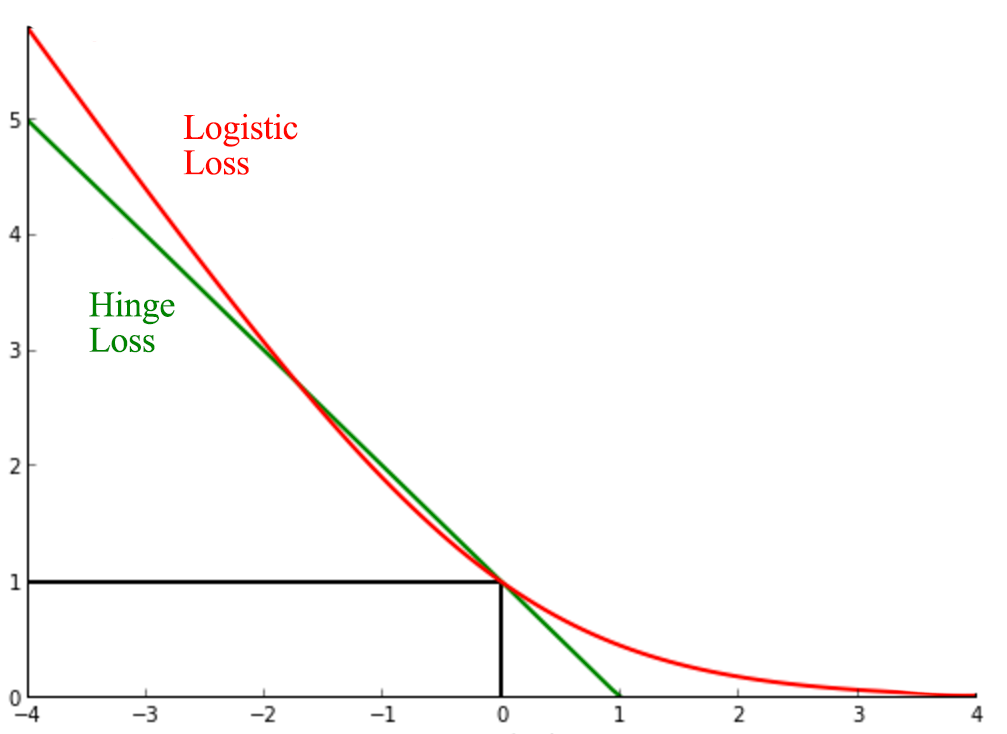
\includegraphics[width=0.4\textwidth]{images/losses-graph.png}
    \caption{Binary, Hinge, and logistic loss for $y'=1$}
\end{wrapfigure}
This loss function is however not convex in $\beta$; therefore, the problem of minimizing $\emrisk_n$ is extremely hard to solve. 
The idea of logistic regression consists in replacing the binary loss with another similar loss function, which is convex in $\beta$. This is the case of both the \emph{Hinge loss} and the \emph{logistic loss} which we will now introduce.

\begin{definition}[Hinge loss]
    The \emph{Hinge loss} $\ell_H:\R\times\{-1, 1\}\to\R_+$ is such that it values to $0$ when both arguments have the same sign and that $|y|\geq1$ (confident prediction), and increases linearly when their signs differ or when $|y|<1$ (prediction not confident enough):
    \begin{equation}
        \ell_H(y, y') := \max(0, 1-yy')
    \end{equation}
\end{definition}

\begin{definition}[Logistic loss]
    The \emph{logistic loss} $\ell_l:\R\times\{0, 1\}\to\R_+$ is defined by:
    \begin{equation}
        \ell_l(y, y') := y'\log(1-e^{-y}) + (1-y')\log(1+e^y)
    \end{equation}
\end{definition}

The advantage of the logistic loss with respect to the Hinge loss is that it has a probabilistic interpretation, by modeling $\P(Y=1|X)$, where $(X, Y)$ is a couple of random variables following the law $(X_i, Y_i)$. We will see more on this in the lecture on Maximum Likelihood.

\begin{definition}[Logistic regression estimator]
    The logistic regression estimator is the solution of the following minimization problem:
    \begin{equation}
        \hat{\beta}_{\textnormal{(logi.)}} := \argmin_{\beta\in\R^d}\frac{1}{n}\sum_{i=1}^n \ell_l(X^\tp_i\beta, Y_i)
    \end{equation}    
\end{definition}

\subsubsection{Computation of the estimator}
Similarly to OLS, we may try to analyticall solve the minimization problem to find $\hat{\beta}_{(\textnormal{logi.})}$. This could be done by cancelling the gradient of the empirical risk. Note that:
\begin{equation*}
    \frac{\partial\ell_l(y, y')}{\partial y} = \sigma(y)-y'
\end{equation*}
where $\sigma$ is the logistic function
\begin{equation*}
    \sigma = z \longmapsto \frac{1}{1+e^{-z}}.
\end{equation*}
Therefore,
\begin{equation*}
    \nabla\emrisk_n(\beta) = \frac{1}{n}\sum_{i=1}^nX_i(\sigma(X_i^\tp\beta)-Y_i)=\frac{1}{n}X(Y-\sigma(X\beta))
\end{equation*}
where $\sigma(X\beta)_i:=\sigma(X_i^\tp\beta)$. The problem is that the equation $\nabla\emrisk_n(\beta)=0$ had no closed-form solution. Therefore, it needs to be solved through iterative algorithms (gradient descent, Newton's method, \dots). Fortunately, this is possible, since the logistic loss is convex in its first argument. Indeed:
\begin{equation*}
    \frac{\partial^2\ell_l(y, y')}{\partial y^2} = \sigma(y)\sigma(-y)>0
\end{equation*}
Furthermore, the loss being strictly convex, the solution is even unique. In this chapter and in the next one, we will see tools and methods to solve convex optimization problems.

\subsubsection{Regularization}
Similarly to linear regression, logistic regression may over-fit the data (especially when $p>n$). In this case, one needs to add a regularization term, such as $\lambda\norm{\beta}^2_2$ to the logistic loss.

\subsection{Convex analysis}
\subsubsection{Convexity and minimization problems}
We will now see notions of convex analysis to solve convex optimization problems, such as logistic regression. This chapter will introduce convex analysis -- the properties of convex functions and convex optimization problems, and the next chapter will approach convex optimization algorithms (gradient descent, Newton's method, stochastic gradient descent, \dots).
\begin{wrapfigure}[10]{l}{0.4\textwidth}
    \centering
    \captionsetup{justification=centering}
    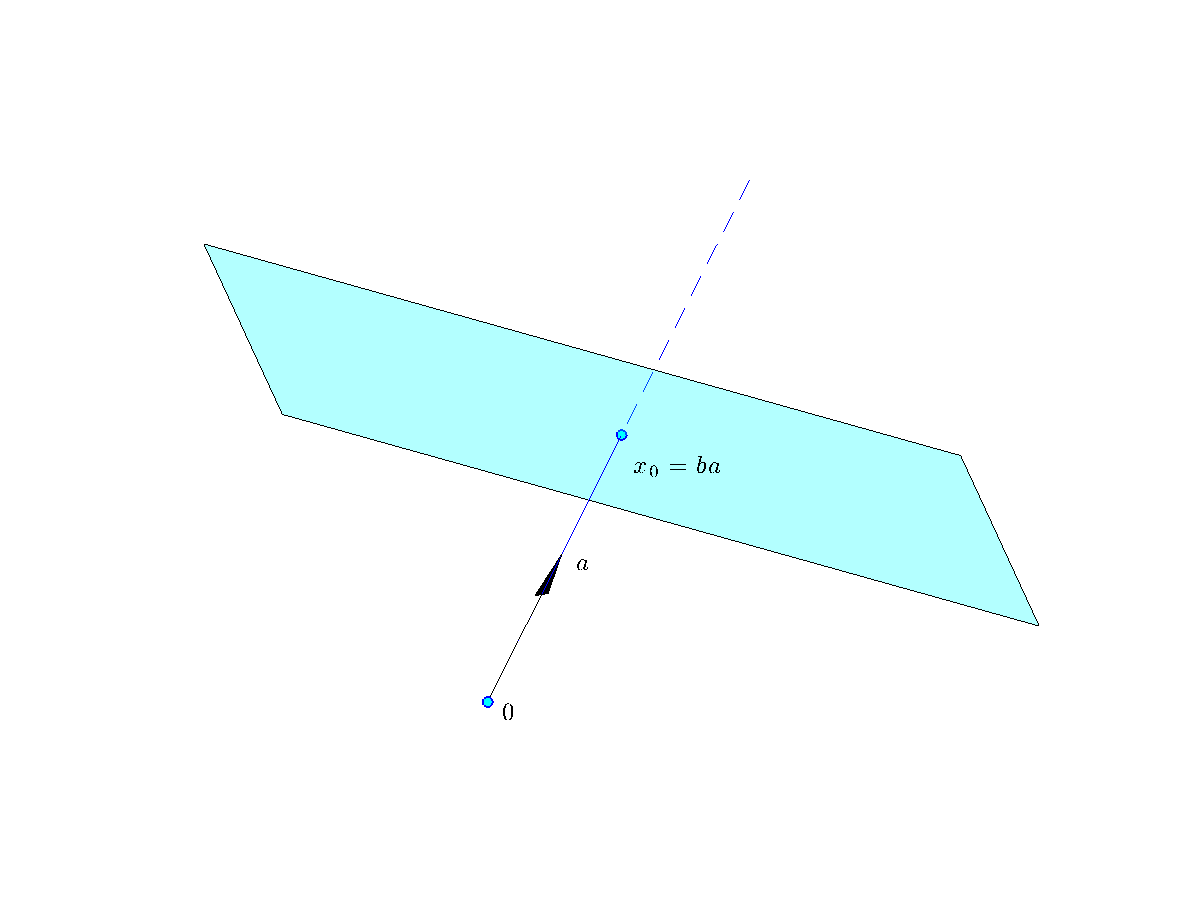
\includegraphics[width=0.3\textwidth]{images/hyperplane.png}
    \caption{Hyperplane}
\end{wrapfigure}

Convexity is a crucial notion in many fields of mathematics and computer science. In machine learning, convexity creates well-defined problems with efficient solutions. A typical example is the problem of \emph{empirical risk minimization}:
\begin{equation*}
    \hatf_n\in\argmin_{f\in\mathcal{F}}\frac{1}{n}\sum_{i=1}^n\ell(f(X_i), Y_i)+\lambda\Omega(f)
\end{equation*}
where $D_n=\set{(X_i, Y_i)}{i\in\iset{1}{n}}$ is the data set, $\mathcal{F}$ is a \emph{convex} set of predictors $f:\X\to\R$, for all $y'\in\Y$, $y\mapsto\ell(y, y')$ is a convex loss function, and $\Omega$ is a convex penaly (such as $\norm{\cdot}_2$, $\norm{\cdot}_1$, \dots).

Convexity will be useful to analyze bot statistical properties of the solution $\hatf_n$ and its generalization error:
\begin{equation*}
    \risk(\hatf_n):=\E[\ell(f(X), Y)|D_n]
\end{equation*}
but also to derive efficient algorithms to solve the forementionned minimization problem and find $\hatf_n$.

\subsubsection{Convex sets}
In what follows, we will only consider finite dimensional Euclidean spaces (typically $\R^d$).
\begin{wrapfigure}{r}{0.4\textwidth}
    \centering
        \captionsetup{justification=centering}
        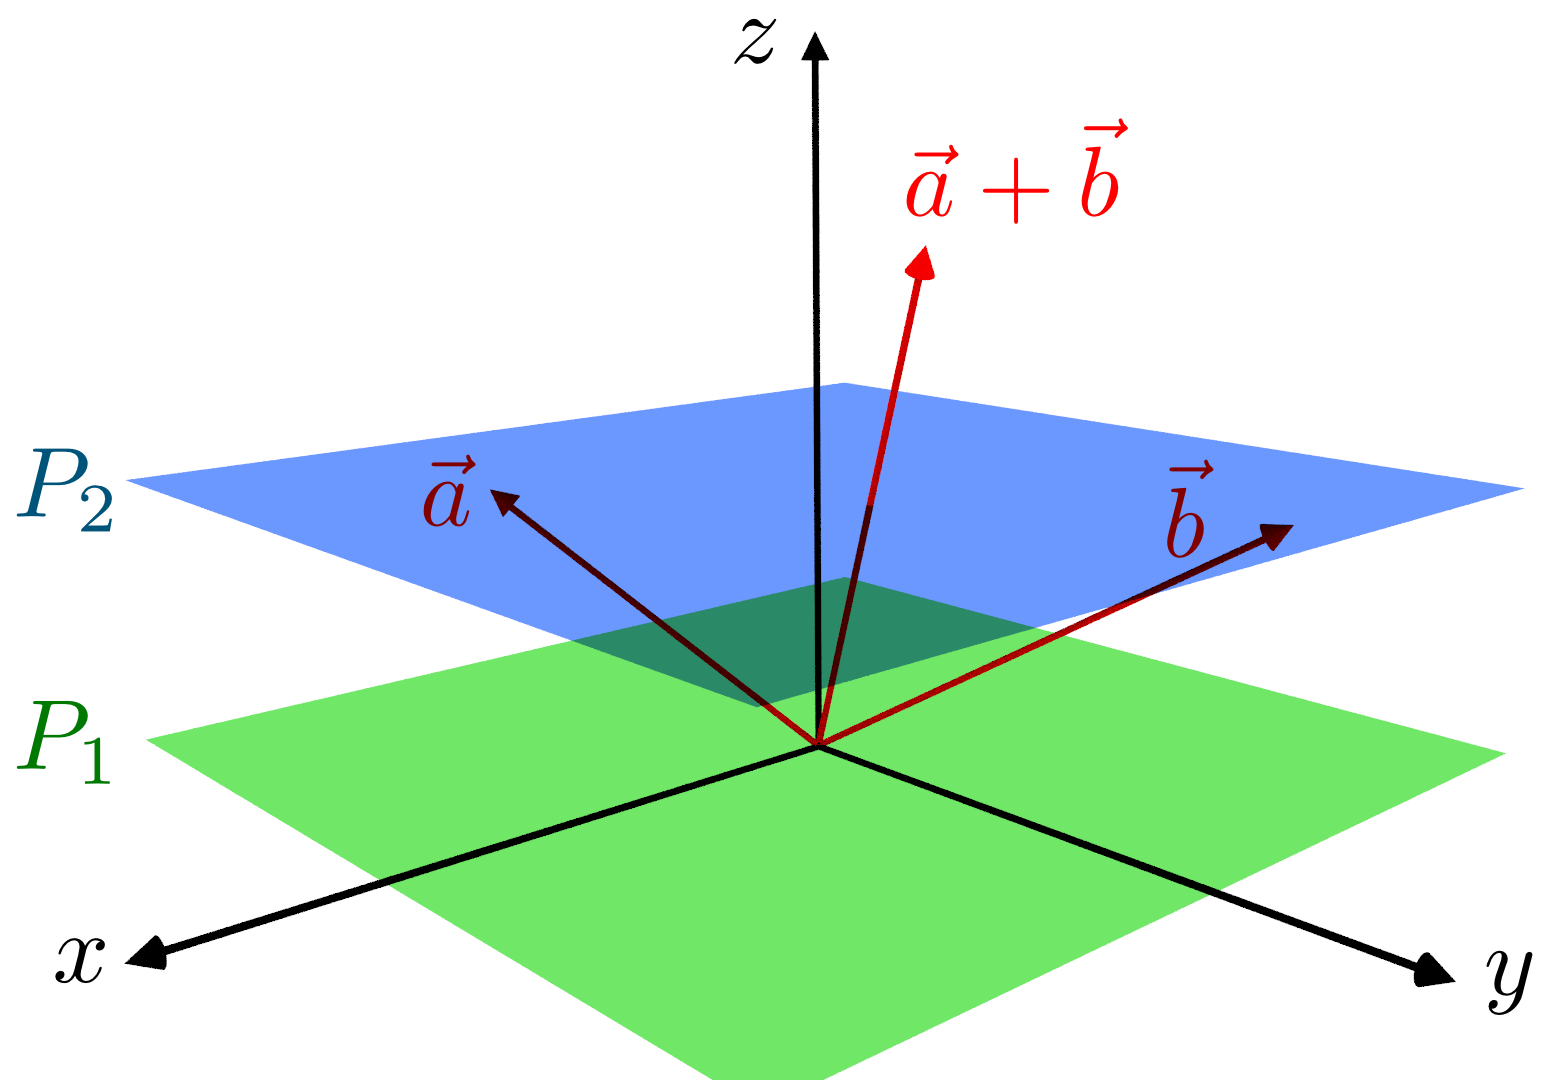
\includegraphics[width=0.35\textwidth]{images/affine-space.png}
        \caption{Affine space}
\end{wrapfigure}


\begin{definition}[Convex set]
    A set $K\subseteq\R^d$ is convex if and only if:
    \begin{equation*}
        \forall x, y\in K, \forall \alpha\in[0, 1], \quad \alpha x+(1-\alpha)y \in K
    \end{equation*}
    Said otherwise, $K$ is stable by barycentration, or, for all points $x, y\in K$, $[x, y]\subseteq K$.
\end{definition}

\begin{example}
    The following sets are convex:
    \begin{itemize}
        \item Hyperplans: $K=\set{x\in\R^d}{a^\tp x = b, a\neq 0, b\in\R}$
        \item Half spaces: $K=\set{x\in\R^d}{a^\tp x\geq b, a\neq0, b\in\R}$
        \item Affine subspaces: $K=\set{x\in\R^d}{Ax=b, A\in\mathscr{M}_d(\R), b\in\R}$
        \item Balls: $\set{x\in\R^d}{\norm{x}\leq R}$
        \item Cones: $K=\set{(x, r)\in\R^{d+1}}{\norm{x}\leq r}$
        \item Convex polytopes: intersections of half spaces
    \end{itemize}
\end{example}

\begin{wrapfigure}{l}{0.3\textwidth}
    \centering
        \captionsetup{justification=centering}
        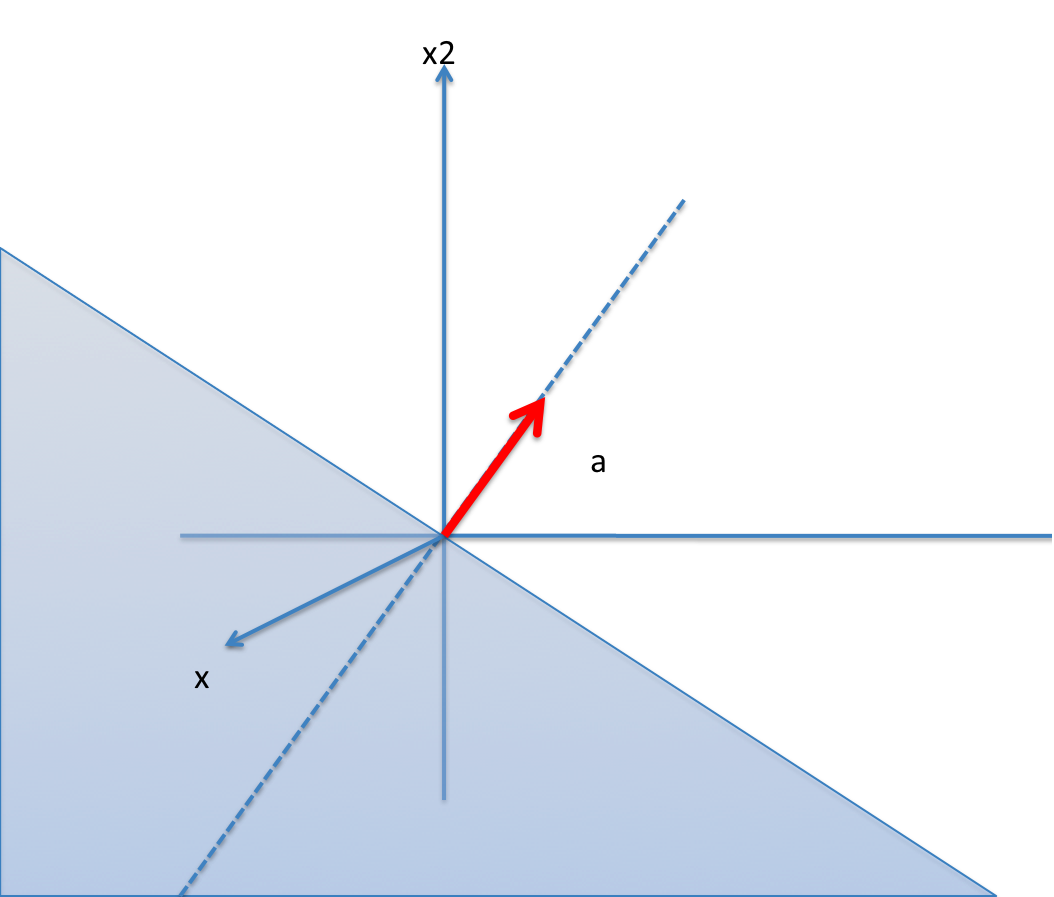
\includegraphics[width=0.3\textwidth]{images/half-space.png}
        \caption{Half-space}
\end{wrapfigure}
We know ennounce useful properties of convex sets.
\begin{property}[Stability by intersection]
    Convexity is stable by intersection. If $(K_i)_{i\in I}$ is a collection -- non-necessarily countable -- of convex sets, then:
    \begin{equation*}
        \bigcap_{i\in I}K_i \quad\textnormal{is convex}
    \end{equation*}
\end{property}

\begin{property}[Stability by affine transformation]
    Convexity is stable by affine transformation. If $K\subseteq\R^d$ is a convex set, then for all $\lambda\in\R$ and $\beta\in \R^d$,
    \begin{equation*}
        \lambda\cdot K+\beta := \set{\lambda\cdot x+\beta}{x\in K} \quad \textnormal{is convex}
    \end{equation*}
\end{property}

\begin{property}[Convex serparation]
    If $C$, $D$ are disjoints convex sets (i.e. $C\cap D=\emptyset$), then there exists a hyperplane which separates $C$ and $D$:
    \begin{equation*}
        \exists a\neq0, b\in\R, \quad C\subseteq\set{x\in\R^d}{a^\tp x\geq b}, D\subseteq\set{x\in\R^d}{a^\tp x\leq b}
    \end{equation*}
    Moreover, the inequalities are strict if $C$ and $D$ are compact.
\end{property}

\begin{wrapfigure}{r}{0.3\textwidth}
    \centering
        \captionsetup{justification=centering}
        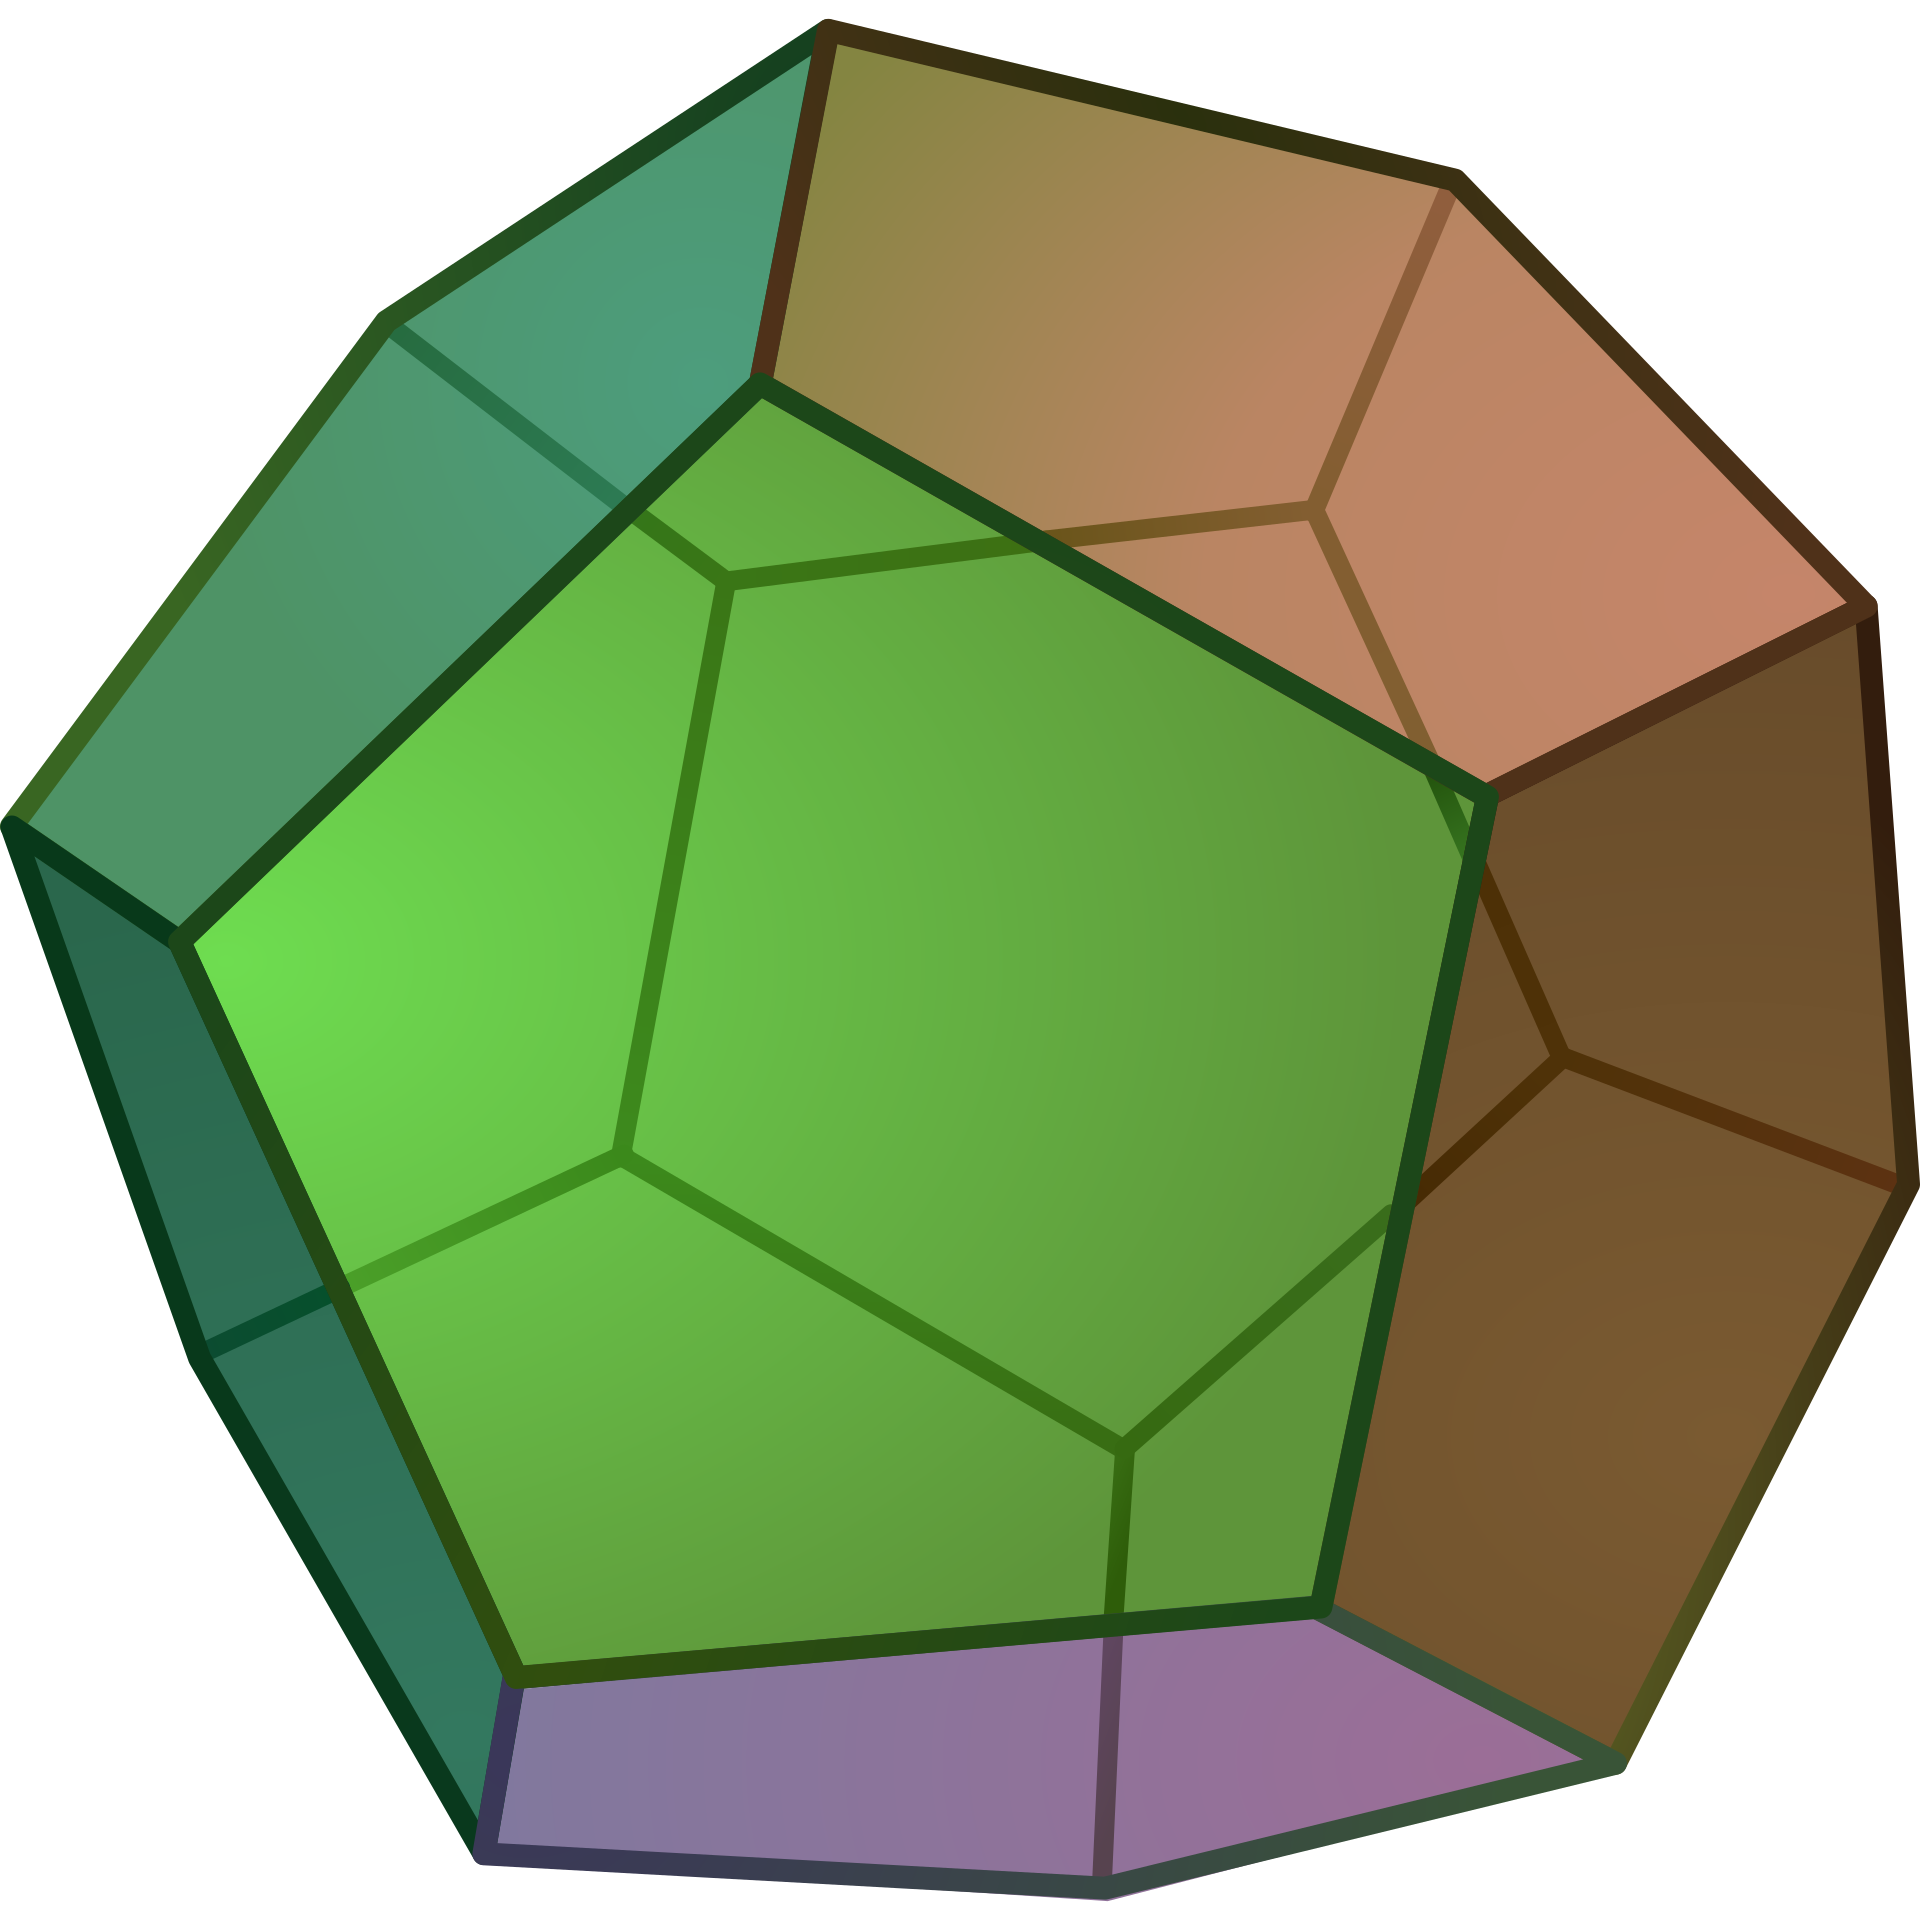
\includegraphics[width=0.2\textwidth]{images/polytope.png}
        \caption{Polytope}
\end{wrapfigure}
When a set is not convex, a trick is to use its convex hull to show some properties on it.
\begin{definition}[Convex Hull]
    Let $A\in\R^d$. The \emph{Convex Hull} of $A$, denoted $\Conv(A)$, is the smallest convex set that contains $A$. In other words,
    \begin{equation*}
        \begin{aligned}
            \Conv(A):=&\,\bigcap\set{B\in\R^d}{A\subseteq B, B \textnormal{ convex}}\\
            =&\,\set{\sum_{i=1}^p\alpha_iz_i}{p\geq 1, \alpha\in\R_+^p, (z_1, \dots, z_p)\in A^p, \; \sum_{i=1}^p \alpha_i=1}
        \end{aligned}
    \end{equation*}
\end{definition}

\subsubsection{Convex functions}
\begin{definition}[Convex function]
    A function $f:D\subseteq\R^d\to\R$ where $D$ is convex is a \emph{convex function} when:
    \begin{equation}
        \forall x, y \in D, \forall \alpha\in[0, 1], \quad f(\alpha x+(1-\alpha)y)\leq\alpha f(x) + (1-\alpha)f(y)
    \end{equation}
\end{definition}

\begin{definition}[Stricly convex function]
    A function $f:D\subseteq\R^d\to\R$ where $D$ is convex is a \emph{strictly convex function} when:
    \begin{equation}
        \forall x, y \in D, \forall \alpha\in[0, 1], \quad f(\alpha x+(1-\alpha)y)<\alpha f(x) + (1-\alpha)f(y)
    \end{equation}
\end{definition}

\vspace*{-0.5cm}
\begin{figure}[H]
    \centering
    \captionsetup{justification=centering}
    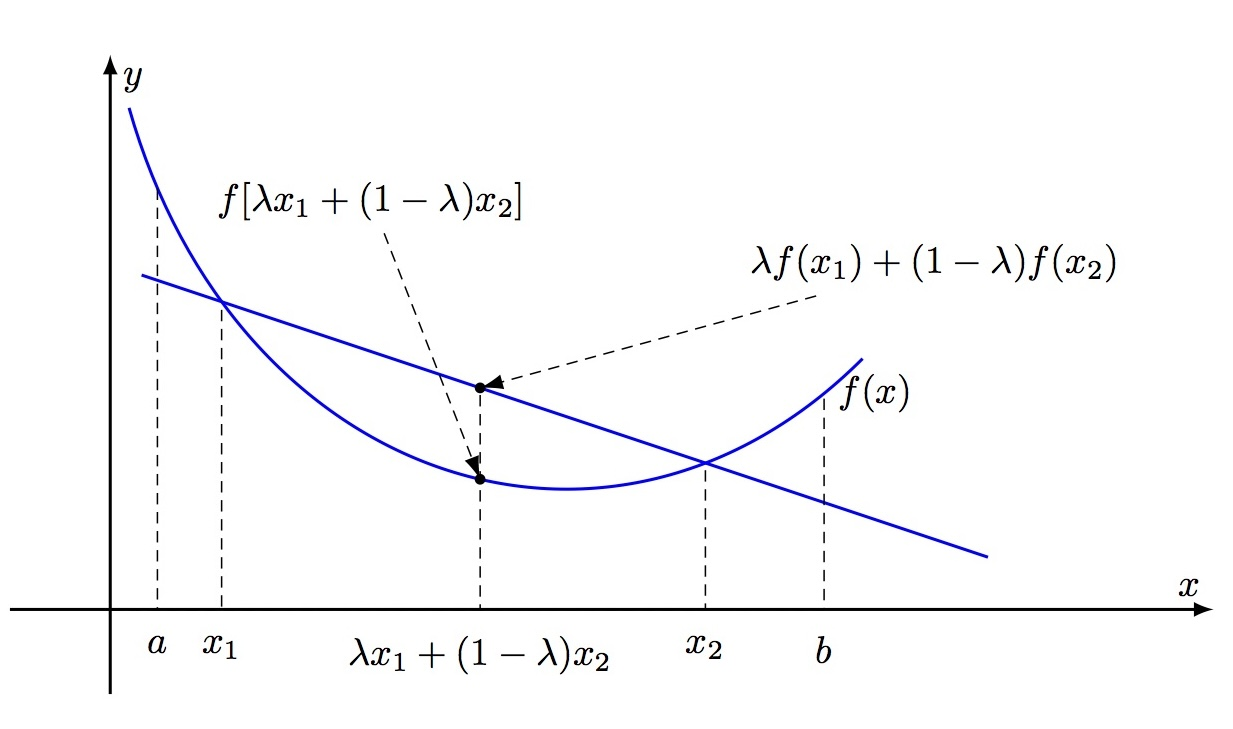
\includegraphics[width=0.7\textwidth]{images/convexity.jpg}
    \caption{Geometric interpretation of convexity}
\end{figure}

\begin{definition}
    A function $f:D\subseteq\R^d\to\R$ where $D$ is convex is \emph{$\mu$-stricly convex} when 
    \begin{equation*}
        x\longmapsto f(x)-\frac{\mu}{2}\norm{x}^2 \quad\textnormal{is convex}
    \end{equation*}
\end{definition}

\begin{example}[Convex functions]
    \leavevmode
    All the following functions are convex:
    \begin{figure}[H]
        \centering
        \begin{tabular}{c c}
            \begin{minipage}{0.45\textwidth}
                \vspace*{-0.4cm}
                In dimension $d=1$:
                \begin{itemize}
                    \item $x\longmapsto x$
                    \item $x\longmapsto x^2$
                    \item $x\longmapsto -\log(x)$
                    \item $x\longmapsto \log(1+e^{-x})$
                    \item $x\longmapsto |x|^p$ for $p\geq1$
                    \item $x\longmapsto -x^p$ for $p<1$
                \end{itemize}
            \end{minipage}
            \begin{minipage}{0.5\textwidth}
                Higher dimensions $d\geq1$:
                \begin{itemize}
                    \item Linear functions $x\longmapsto aa^\tp x$
                    \item Quadratic functions $x\longmapsto x^\tp Qx$ for $Q$ semidefinite symmetric positive matrix
                    \item Norms
                    \item $x\longmapsto\max\set{x_i}{i\in\iset{1}{d}}$
                    \item $x\longmapsto\log\left(\sum_{i=1}^de_i^x\right)$
                \end{itemize}
            \end{minipage}
        \end{tabular}
    \end{figure}
\end{example}

In practice, the functions which we will consider will be $\mathcal{C}^1$ and even $\mathcal{C}^2$. In this case, much simpler characterization are given for convex functions.

\begin{property}[Differentiable convex functions]
    If $f$ is $\mathcal{C}^1$,
    \begin{equation*}
        f \textnormal{ convex} \iff \forall x, y\in D, f(x)\geq f(y) + f'(y)(x-y)
    \end{equation*}
\end{property}
\begin{property}[Twice differentiable convex functions]
    If $f$ is twice differentiable,
    \begin{center}
        $f$ convex $\iff$ $\forall x\in D$, its Hessian is semi-definite positive ($f''(x)\geq0$)
    \end{center}
\end{property}

\begin{property}[Operations which preserve convexity]
    If $(f_i)_{i\in I}$ is a family of convex functions, then,
    \begin{equation*}
        x \longmapsto \sup_{i\in I} f_i(x) \quad\textnormal{is convex}
    \end{equation*}
    \begin{equation*}
        \forall \alpha_i\in\R_+, x \longmapsto \sum_{i\in I} \alpha_i f_i(x) \quad\textnormal{is convex}
    \end{equation*}
    Furthermore, if $f$ is convex on $C\times D$, then
    \begin{equation*}
        y \longmapsto \inf_{x\in C} f(x, y) \quad \textnormal{is convex on $D$}
    \end{equation*}
\end{property}

\begin{property}[Convexity and continuity]
    If $f$ is convex on $D$, then $f$ is continuous on $\mathring{D}$. Furthermore, the epigraph of $f$,
    \begin{equation*}
        \set{(x, t)\in D\times\R}{f(x)\leq t} \quad \textnormal{is convex.}
    \end{equation*}
\end{property}

\begin{property}[Jensen's inequality]
    For $f$ convex, $x_1, \dots, x_n\in D$ and $\alpha_1,\dots, \alpha_n\in\R_+$ such that $\sum_{i=1}^n\alpha_i=1$. Then:
    \begin{equation*}
        f\left(\sum_{i=1}^n\alpha_ix_i\right) \leq \sum_{i=1}^n\alpha_if(x_i)
    \end{equation*}
\end{property}

\begin{property}[Jensen's integral inequality]
    For $f$ convex, $p(x)\geq0$ over $S\subseteq D$ such that $\int_s p(x)\,\textnormal{d}x=1$, then:
    \begin{equation*}
        f\left(\int_Sp(x)\,\textnormal{d}x\right) \leq \int_Sp(x)f(x)\,\textnormal{d}x
    \end{equation*}
\end{property}

\begin{property}[Jensen's expectation inequality]
    For $f$ convex, and $X$ a random variable such that $X\in D$ almost surely and with $\E[X]<+\infty$, then:
    \begin{equation*}
        f(\E[X])\leq\E[f(X)]
    \end{equation*}
\end{property}

\subsubsection{Unconstrained optimization problems}
Let $f:\R^d\to\R$ be a convex function. We consider the following minimization problem:
\begin{equation*}
    \inf_{x\in\R^d}f(x)
\end{equation*}
Note that the notation $\min_x f(x)$ is only used when the minimum is reached. If no point achieves the minimum, we use the notation $\inf_xf(x)$.

Three cases are possible, depending on $\inf_xf(x)$:
\begin{itemize}
    \item $\inf_{x\in\R^d}f(x)=-\infty$ -- there is no minimum.
    \item $\inf_{x\in\R^d}f(x)>-\infty$ and the minimum is not reached.
    \item $\inf_{x\in\R^d}f(x)>-\infty$ and the minimum is reached and equals $\min{x\in\R^d}f(x)$.
\end{itemize}

\begin{definition}[Local minimum]
    Let $f:D\to\R$ and $x\in D$. $x$ is a local minimum if and only if there exists an open set $V\subseteq D$ such that $x\in V$ and $f(x)=\min_{x'\in V}f(x')$.
\end{definition}

\begin{property}
    \label{prop:local-global-min}
    If $f$ is convex, any local minimum of $f$ is a global minimum.
\end{property}

\begin{property}
    If $f$ is stricly convex, it has at most one minimum.
\end{property}

\begin{property}
    If $f$ is convex and $\mathcal{C}^1$, then $x$ is a minimum of $f$ on $\R^d$ if and only if $f'(x)=0$.
\end{property}

\begin{figure}[H]
    \centering
    \captionsetup{justification=centering}
    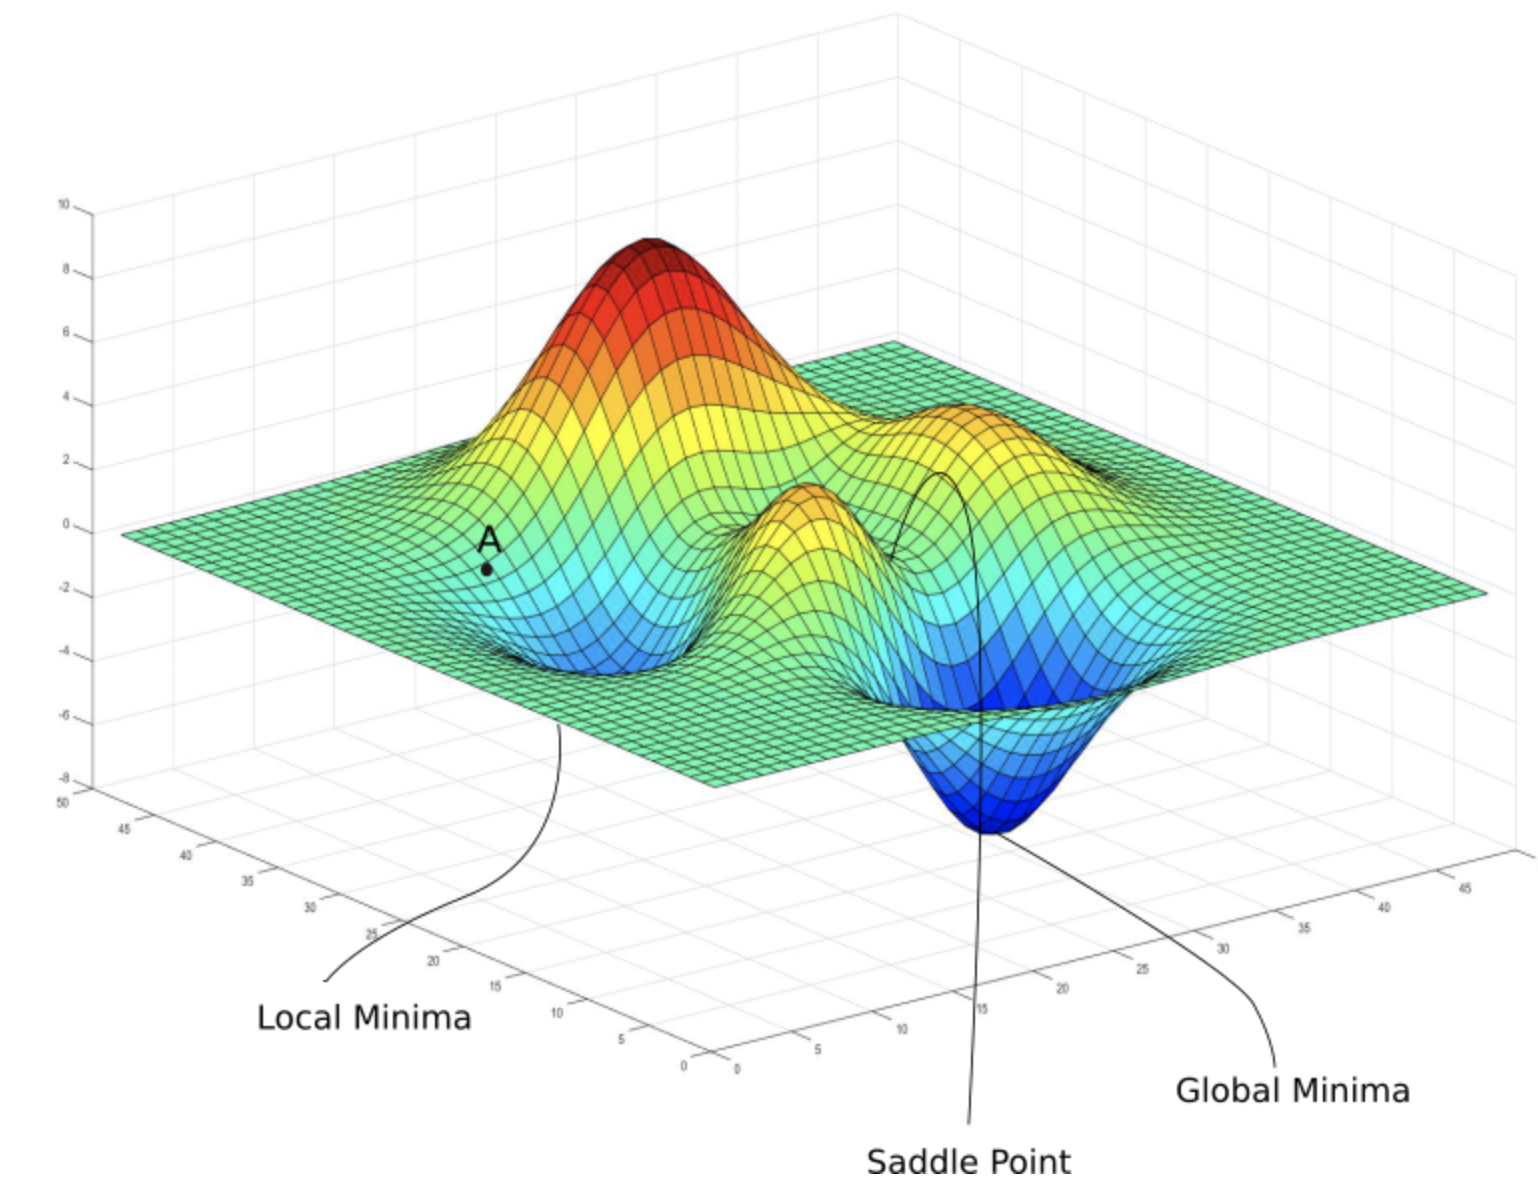
\includegraphics[width=0.7\textwidth]{images/local-minimum.png}
    \caption{Local and global minima of a non-convex function}
\end{figure}
These three properties justify the apprach of canceling the gradient to efficiently find a solution to a minimization problem. Property \ref{prop:local-global-min} guarantees that the result of some gradient descent is a global minimum, and not just some dead-end for the descent path. Strict convexity guarantees that every converging gradient descent will end up at the same minimum.

In the next chapter, we will continue the analysis of this frequent minimization problem and develop formal tools and algorithm to solve it efficiently.

\section{Convex analysis and convex optimization}
\subsection{Constrained optimization problems}
Let $f:D\mapsto\R^d$ convex and $C\subseteq D$ convex. We consider the constrained minimization problem
\begin{equation*}
    \inf_{x\in C}f(x)
\end{equation*}
where $C$ is the constraint set. It is often  defined as the intersection of sets of the form $\set{h_i(x)=0}{i\in I}$ (hyperplanes) and $\set{g_j(x)\leq0}{j\in J}$ (half-spaces).

\begin{example}[Minimization of a linear function over a compact]
    Let $A\subseteq\R^d$ be a compact, non-necessarily convex set, and $a\in\R^d\setminus\{0\}$. We can reformulate the non-convex minimization problem on $A$ as a constrained convex optimization problem on $\Conv(A)$:
    \begin{equation*}
        \min\set{a^\tp x}{x\in A} = \min\set{a^\tp x}{x\in\Conv(A)}
    \end{equation*}    
\end{example}

\subsubsection{Lagrangian duality}
A useful notion to solve constrained problems is Lagrangian duality. Assume that we are interested in the following constrained optimization problem:
\begin{equation}
    \label{eq:optimization-problem}
    \min_{x\in D}f(x) \quad \textnormal{such that}\quad 
    \begin{cases*}
        \tag{P}
        h_i(x) = 0 & for $i\in\iset{1}{m}$\\
        g_j(x)\leq0 & for $j\in\iset{1}{r}$
    \end{cases*}
\end{equation}
We denote by $D^*\subseteq D$ the set of points that satisfy the constraints:
\begin{equation*}
    D^* := \set{x\in D}{\forall i\in\iset{1}{m}, h_i(x)=0 \land \forall j\in\iset{1}{r}, g_j(x)\leq 0}
\end{equation*}
Note that the equality constraints $h_i(x)=0$ can be rewritten as inequalities:
\begin{equation*}
    h_i(x)\leq0 \land -h_i(x)\leq0
\end{equation*}
Unlike unconstrained optimization problems, canceling the gradient does not necessarily provide a solution for constrained optimization problems. The basic idea of Lagrangian duality is therefore to take the constraint $D^*$ into account in the minimization problem by augmenting the objective function with a weighted sum of the constraint functions.

\begin{figure}
    \centering
    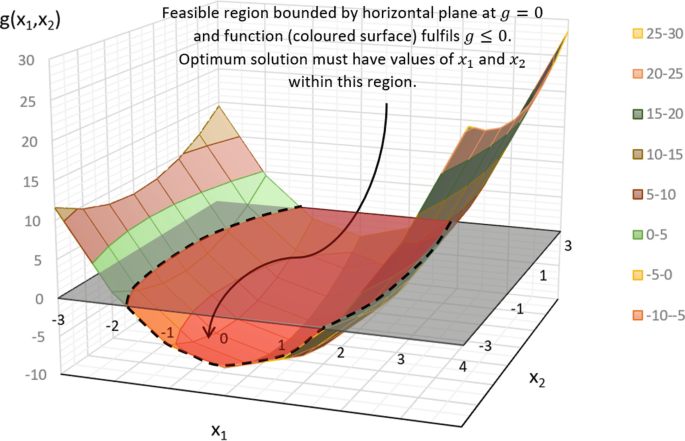
\includegraphics[width=0.7\textwidth]{images/constrained-optimization.png}
    \caption{Constrained optimization: $D^*$ is the red and orange part below the $g$ plane}
\end{figure}

\begin{definition}[Lagrangian]
    The \emph{Lagrangian} associated to the optimization problem \eqref{eq:optimization-problem} is the function
    \begin{equation*}
        \L:D\times\R^m\times\R_+^r \longrightarrow \R
    \end{equation*}
    defines by:
    \begin{equation*}
        \L(x, \lambda, \mu) = f(x) + \lambda^\tp h(x) + \mu^\tp g(x)
    \end{equation*}
\end{definition}

\begin{definition}[Primal function]
    We define the \emph{primal function} associated to \eqref{eq:optimization-problem}
    \begin{equation*}
        \bar{f}:D\longrightarrow\R\cup\{+\infty\}
    \end{equation*}
    by:
    \begin{equation*}
        \bar{f} : x \longmapsto \sup_{\lambda\in\R^m, \;\mu\in\R^r_+} \L(x, \lambda, \mu) = \begin{cases*}
            f(x) & if $x\in D^*$\\
            +\infty & otherwise
        \end{cases*}
    \end{equation*}
\end{definition}

\begin{definition}[Primal problem]
    With these definitions, we observe that the optimization problem \eqref{eq:optimization-problem} can be re-written as a constraints-free problem of minimization of the primal function.
    \begin{equation*}
        \begin{aligned}
            \inf_{x\in D^*} &= \inf_{x\in D}\bar{f}(x)\\
            &= \inf_{x\in D} \sup_{\lambda\in\R^m, \;\mu\in\R^r_+} \L(x, \lambda, \mu)
        \end{aligned}
    \end{equation*}
\end{definition}

\begin{definition}[Dual problem]
    The \emph{Dual problem} is obtained by exchanging inf and sup in the primal problem:
    \begin{equation*}
        \sup_{\lambda\in\R^m, \;\mu\in\R^r_+} f^*(\lambda, \mu) := \sup_{\lambda\in\R^m, \;\mu\in\R^r_+} \inf_{x\in D}\L(x, \lambda, \mu)
    \end{equation*}
    where
    \begin{equation*}
        f^* : (\lambda, \mu) \longmapsto \inf_{x\in D}\L(x, \lambda, \mu)
    \end{equation*}
    is the \emph{dual function}. If $f$ is convex, this function is concave. Note that the dual of the dual is the primal.
\end{definition}

The admissibility domain of the primal is $D^* := \set{x\in D}{\bar{f}(x)<+\infty}$, and the admissibility domain of the dual is $C^* := \set{(\lambda, \mu)\in\R^m\times\R_+^r}{f^*(\lambda, \mu)>-\infty}$. There is no solution to the optimization problem when $D^*=\emptyset$. The problem is unbounded when $C^*=\emptyset$.

\subsubsection{Link between primal and dual problems}
The primal and dual problems are not necessarily identical, but have a strong relationship. For any $(\lambda, \mu)$, $f^*(\lambda, \mu)$ provides a lower bound on the solution of \eqref{eq:optimization-problem}. The dual problem finds the best lower bound.

\begin{property}[Weak duality principle]
    \begin{equation*}
        d^* := \sup_{\lambda\in\R^m, \;\mu\in\R^r_+} \inf_{x\in D}\L(x, \lambda, \mu) \leq \inf_{x\in D} \sup_{\lambda\in\R^m, \;\mu\in\R^r_+} \L(x, \lambda, \mu)
    \end{equation*}    
\end{property}
The solution of the dual problem is therefore always smaller than the solution of the primal. A good mnemonic is to remember this inequality as \say{the largest dwarf is always smaller than the smallest giant}.

\begin{definition}[Dual gap]
    The \emph{dual gap} of the optimization problem is the difference between the primal and dual solutions:
    \begin{equation*}
        p^*-d^* \geq 0
    \end{equation*}
\end{definition}

\begin{definition}[Strong duality]
    There is \emph{strong duality} when $p^*=d^*$. In this case, the two problems are equivalent -- they share the same solutions. The existence of the solultions are related with the existence of saddle point of the Lagrangian. Note that strong duality does not always hold.
\end{definition}

\subsubsection{Strong duality}
Sometimes, the dual problem is easier to solve than the primal problem. It is then useful to know if there is strong duality.

\begin{definition}[Strictly feasible point]
    A point $x_0\in D$ is \emph{strictly feasible} when:
    \begin{equation*}
        \exists x_0\in D, \quad \begin{cases*}
            h_i(x_0)=0 & $\forall i\in\iset{1}{m}$\\
            g_j(x_0)<0 & $\forall j\in\iset{1}{r}$
        \end{cases*}
    \end{equation*}
\end{definition}

\begin{theorem}[Slater's condition]
    If $f$ and $D$ are convex, $h_i$ are affine and $g_j$ are convex, then the existence of a strictly feasible point implies strong duality.
\end{theorem}

\begin{example}
    Let $D=\R^d_+$ and consider the following linear programming minimization problem:
    \begin{equation*}
        \min_{x\in D, \; Ax=b}c^\tp x
    \end{equation*}
    where $A\in\mathscr{M}_{m, d}(\R)$ and $b\in\R^m$. The constraints can be written as $Ax-b=0$. Therefore, the Lagrangian is:
    \begin{equation*}
        \L : (x, \lambda) \in \R_+^d \times \R^m \longrightarrow c^\tp x + \lambda^\tp(b-Ax)
    \end{equation*}
    The primal problem can be rewritten using the Lagrangian:
    \begin{equation*}
        \begin{aligned}
            \min_{x\in D, \; Ax=b}c^\tp x &= \min_{x\in D}\sup_{\lambda\in\R^m} c^\tp x+\lambda^\tp(b-Ax)\\
            &= \min_{x\in D}\sup_{\lambda\in\R^m} b^\tp\lambda+x^\tp(c-A^\tp\lambda)
        \end{aligned}
    \end{equation*}
    The problem is convex since the objective function is convex, and the equality constraints are affine. By Slater's condition, we can swap the $\min$ and the $\sup$, giving:
    \begin{equation*}
        \begin{aligned}
            \min_{x\in D, \; Ax=b}c^\tp x &= \sup_{\lambda\in\R^m} \min_{x\in D} c^\tp x+\lambda^\tp(b-Ax)\\
            &= \sup_{\lambda\in\R^m, \; A^\tp\lambda\leq c} b^\tp\lambda
        \end{aligned}
    \end{equation*}
    This is the dual formulation of the problem.
\end{example}

\subsubsection{Karush-Kuhn-Tucker optimality conditions}
We will now see conditions playing the same role as gradient cancelling for unconstrained optimization problems. These conditions will be useful to find equations to compute analytically the solutions of the minimization problem.

Assume that the function $f$, $h_i$, and $g_i$ are all differentiable. Let $x^*$, and $(\lambda^*, \mu^*)$ be any primal and dual solutions, and assume that there is strong duality.

\begin{property}[KKT1]
    Since $x^*$ minimizes $\L(x, \lambda^*, \mu^*)$ over $x$, its gradient must be canceled at $x^*$:
    \begin{equation}
        \tag{KKT1}
        \nabla f(x^*) + \sum_{i=1}^m \lambda_i^*\nabla h(x^*) + \sum_{j=1}^r\mu_j\nabla g_j(x^*)=0
    \end{equation}
\end{property}

\begin{property}[KKT2]
    Since $x^*\in D^*$ and $(\lambda^*, \mu^*)\in C^*$ are feasible we have:
    \begin{equation}
        \tag{KKT2}
        \begin{aligned}
            \forall i\in\iset{1}{m},& \quad h_i(x^*)=0\\
            \forall i\in\iset{1}{r},& \quad g_j(x^*)\leq0\\
            \forall j\in\iset{1}{r},& \quad \mu_j^*\geq0
        \end{aligned}
    \end{equation}
\end{property}

\begin{property}[KKT3]
    The \emph{complementary condition} holds, i.e.:
    \begin{equation}
        \tag{KKT3}
        \forall j\in\iset{1}{r}, \quad \mu^*_jg_j(x^*)=0
    \end{equation}
\end{property}
\begin{proof}
    By contradiction, if the complementary condition does not hold, we could improve $\mu^*$ by setting $\mu_j^*=0$, since $g_j(x^*)\leq0$ and $(\lambda^*, \mu^*)$ maximizes $\L(x^*, \lambda, \mu)$.
\end{proof}

These conditions are called the Karush-Kuhn-Tucker (KKT) conditions. When the primal problem is convex, these conditions are also sufficient.

\begin{theorem}[Karush–Kuhn–Tucker theorem]
    If there is strong duality, then:
    \begin{center}
        (KKT) conditions are satisfied $\iff$ $\begin{cases*}
            x^* &is a solution to the primal problem\\
            (\lambda^*, \mu^*) & is a solution of the dual problem
        \end{cases*}$
    \end{center}
\end{theorem}

The KKT conditions play an important role in optimization. In some cases, it is possible to solve them analytically. Many optimization methods are conceived for solving the KKT conditions.

\subsection{Optimization algorithms for unconstrained convex optimization}
In this section we will see two widely used optimization algorithms for the problem of unconstrained optimization, \emph{Gradient descent} and \emph{Stochastic Gradient descent}.

Since the goal of minimizing a function $f:\R^d\to\R$ for $d\in\N$ is to find the point $x$ for which the function has minimum value, the fundamental idea behind gradient descent consists in strating from a given $x_0\in\R^d$ and finding the next point following a descet direction iteratively. In particular, we will consider $f$ to be a convex function.

\subsubsection{Gradient Descent}
\begin{wrapfigure}[15]{l}{0.45\textwidth}
    \captionsetup{justification=centering}
    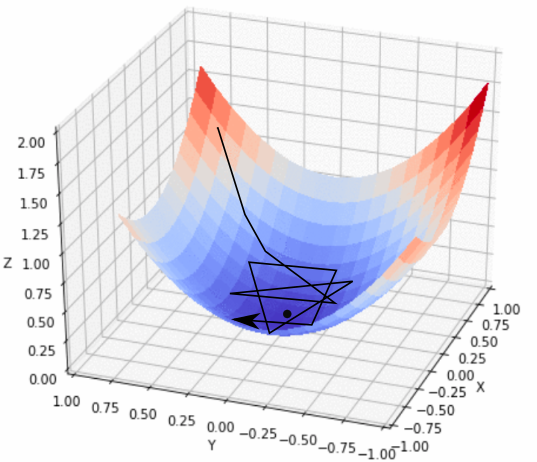
\includegraphics[width=0.4\textwidth]{images/gradient-descent-2.png}
    \caption{Convex gradient descent}
\end{wrapfigure}
When $f$ is diffenrentiable, the gradient of $f$ in $x$, denoted $\nabla f(x)$, determines the direction of maximum increase of the function in a suitable neighborhood of $x$ -- and so $-\nabla f(x)$ determines the direction of maximum decrease of the function. The gradient descent algorithm then reads as follows:
\begin{equation*}
    \begin{cases*}
        x_0 & given\\
        x_{n+1} := x_n -\gamma_n\nabla f(x_n) & $\forall n\in\iset{1}{N}$
    \end{cases*}
\end{equation*}
where $\gamma_n$ is denoted as \emph{step-size} and is small enough such that $-\gamma_n\nabla f(x_n)$ is still a decrease direction in the neighborhood of $x_n$.

The choice of $\gamma_n$ is crucial for the optimization algorithm. If $\gamma_n$ is too big, it makes the algorithm unstable and possibly divergince, since it follows the direction $-\nabla f(x_n)$ out of the region where it is a descent direction. On the other hand, if $\gamma_n$ is too small, the chosen direction is a descent direction, but each step is very short, leading to a larger number of steps required to arrive to the minimum solution -- with a big impact on the total computational complexity.

\begin{figure}[H]
    \centering
    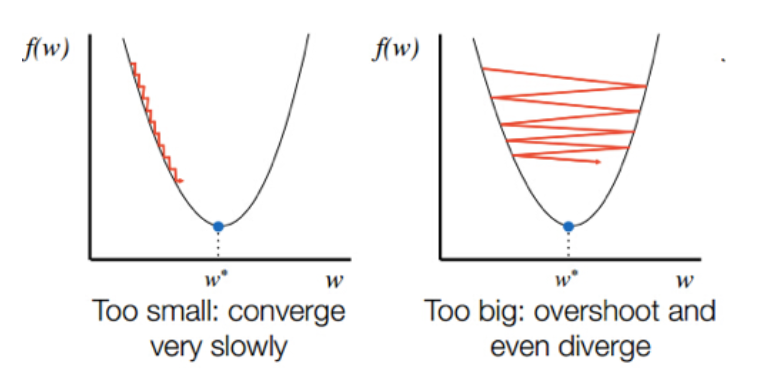
\includegraphics[width=0.7\textwidth]{images/gd-step-size.png}
    \caption{Choice of step size}
\end{figure}

We will prove in the next theorem that there exists a step-size that guarantees the convergence of the solution of the gradient descent algorithm to the minimizer of $f$, and we characterize how fast gradient descent achieves it.

\subsubsection{Gradient Descent for strongly convex functions}
\begin{definition}[$L$-Lipschitz continuous gradients]
    For $L>0$, $f$ has $L$-Lipschitz continuous gradients when:
    \begin{equation*}
        \forall x, y, \in\R^d, \quad \norm{\nabla f(x) - \nabla f(y)}\leq L\norm{y-x}
    \end{equation*}
\end{definition}

\begin{lemma}
    Let $L>0$ and $f:\R^d\to\R$ be a convex function with $L$-Lipschitz continuous gradients, then:
    \begin{equation}
        f(y)\leq f(x)+\nabla f(x)^\tp(y-x)+L\norm{y-x}^2
    \end{equation}
\end{lemma}
\begin{proof}
    %TODO
\end{proof}

\begin{remark}
    Using a different argument, it is possible to prove the tighter result:
    \begin{equation*}
        f(y)\leq f(x)+\nabla f(x)^\tp(y-x)+\frac{L}{2}\norm{y-x}^2
    \end{equation*}
\end{remark}

\begin{lemma}[Gradient descent is a descent algorithm with $\gamma_n\in\rbrack 0, 1/L\lbrack$]
    Let $f$ be convex with $L$-Lipschitz gradient, let $x_0\in\R^d$ and $\gamma_n>0$, then:
    \begin{equation*}
        \forall n\in\N^*, \quad f(x_n)\leq f(x_{n-1}) - \gamma_n(1-L\cdot\gamma_n) \cdot \norm{\nabla f(x_{n-1})}^2
    \end{equation*}
    In particular, if $\gamma_n\in\rbrack 0, 1/L\lbrack$, we have that $\gamma_n(1-L\cdot\gamma_n)>0$. Therefore, for all $n\in\N^*$:
    \begin{equation*}
        f(x_n)<f(x_{n-1})
    \end{equation*}
    whenever $x_{n-1}$ is not a global optimum, otherwise $x_n=x_{n-1}$ and $f(x_n)=f(x_{n-1})$ (a fixpoint is reached).
\end{lemma}
\begin{proof}
    
\end{proof}

\subsubsection{Stochastic Gradient Descent}

\section{Kernels}
\subsection{Introduction to kernels}
In this course, we often focused on prediction methods which are \emph{linear}, that is, the input data are vectors and the prediction function is linear (e.g. $f(x)=w^\tp x$ for $w\in\R^d$). In this situation with given data $(x_i, y_i)$, the vector $w$ can be obtained by minimizing
\begin{equation*}
    \hat{L}(w)=\frac{1}{n}\sum_{i=1}^n l(y_i, w^\tp x_i) + \lambda \Omega(w)
\end{equation*}

Classical examples are logistic regression or least-squares regression. These methods look at first sight of limited practical significance, because input data may not be vectors, and relevant prediction functions may not be linear.

The goal of kernel methods is therefore to go beyond these limitations while keeping the good aspects. The underlying principle is to replace $x$ by a function $\phi(x)\in\R^d$, \emph{explicitly} or \emph{implicitly}, and consider linear predictions in $\Phi(x)$, i.e.~$f(x)=w^\tp \phi(x)$. We call $\phi(x)$ the \emph{feature} associated to $x$.

\begin{example}[Linear regression]
    In the case of linear regression, $\phi(x)=x$ for $x\in\R^d$. As expected, this gives us linear models:
    \begin{equation*}
        f(x)=w^\tp x = \sum_{j=1}^d w_jx_j
    \end{equation*}
\end{example}

\begin{example}[Polynomial regression of degree $r$]
    With $x\in\R$, we have $\phi(x)\in\R^{r+1}$ defined by:
    \begin{equation*}
        \phi(x)=(1, x, x^2, \dots, x^r)
    \end{equation*}
    Therefore, the prediction functions will be general polynomials of degree at most $r$:
    \begin{equation*}
        f(x)=w^\tp\phi(x)=\sum_{j=0}^r (\phi(x))_j = \sum_{j=1}^r w_jx^j
    \end{equation*}
\end{example}

\begin{example}[Polynomial multivariate regression of degree $r$]
    We consider $x\in\R^d$ and
    \begin{equation*}
        \phi(x)=(x_1^{\alpha_1}, \dots, x_d^{\alpha_d})
    \end{equation*}
    with $\sum_{i=1}^d \alpha_i=r$. In this situation, $p=\binom{d+r-1}{r}$ might be too big for an explicit representation to be feasible;
\end{example}

\begin{example}[Generic set of functions]
    Let $\varphi_1, \varphi_r : \R^d \to \R$ be a set of functions of interest (e.g. a subset of the Fourier basis); we define $\phi(x) = (\varphi_1(x), \dots, \varphi_r(x))$ to have:
    \begin{equation*}
        f(x)=w^\tp \phi(x) = \sum_{j=1}^rw_j\varphi_j(x)
    \end{equation*}
\end{example}

\subsection{Representer theorem}
\subsubsection{Theorem statement}
Given a dataset $x_1, \dots, x_n$, we are able to compute the observed feature maps $\phi_(x_1), \dots, \phi(x_n)$. We can ask ourselves if there exists an easier representation for $w$ in terms of these observed feature maps, i.e.~we want to know if it is possible to characterize the minimum $\hat{w}$ of:
\begin{equation*}
    \hat{L}(w) = \frac{1}{n}\sum_{i=1}^n l(y_i, w^\tp\phi(x_i)) + \lambda w^\tp w
\end{equation*}
in the form of $\hat{w} = \sum_{i=1}^n \alpha_i\phi(x_i)$, with $\alpha_i\in\R$. The following theorem guarantees such characterization under basic properties of $\hat{L}$.

\begin{theorem}[Representer theorem]
    Let $\phi:\X\to\R^d$. Let $(x_1, \dots, x_n)\in\X^n$ and assume that $\Psi:\R^{n+1}\to\R$ is strictly increasing with respect to the last variable. Then, the minimum of
    \begin{equation*}
        \hat{L}(w) := \Psi(w^\tp\phi(x_1), \dots, w^\tp\phi(x_n), w^\tp w)
    \end{equation*}
    is obtained for
    \begin{equation*}
        w=\sum_{i=1}^n \alpha_i \phi(x_i)
    \end{equation*} for some $\alpha\in\R^n$.
\end{theorem}

\begin{proof}
    % TODO
\end{proof}

\begin{corollary}
    For $\lambda>0$, 
    \begin{equation*}
        \min_{w\in\R^d} \frac{1}{n} \sum_{i=1}^n l(y_i, w^\tp\phi(x_i)) + \frac{\lambda}{2} w^\tp w
    \end{equation*}
    is obtained for
    \begin{equation*}
        w = \sum_{i=1}^n \alpha_i\phi(x_i).
    \end{equation*}
\end{corollary}

Note that there is no assumption on $l$, and in particular, no convexity assumption. This result is extendable to Hilbert spaces (RKHS), as we will see in the next section.

\subsubsection{Finite dimensional representation of the learning problem}
Using the representer theorem, we know that the minimum of $\hat{L}$ is of the form $w=\sum_{i=1}^n \alpha_i\phi(x_i)$; we can therefore directly optimize this characterization, i.e.~we can then write:
\begin{equation*}
    \min_{w\in\R^r} \frac{1}{n} \sum_{i=1}^n l(y_i, w^\tp\phi(x_i)) + \frac{\lambda}{2} w^\tp w = \min_{\alpha\in\R^n} \frac{1}{n}\sum_{i=1}^n l(y_i, (K\alpha)_i) + \frac{\lambda}{2}\alpha^\tp K\alpha
\end{equation*}
where $K$ is an $n\times n$ matrix with values
\begin{equation*}
    K_{i, j} = \phi(x_i)^\tp \phi(x_j).
\end{equation*}

Indeed,
\begin{equation*}
    \phi(x_i)^\tp w = \sum_{j=1}^n \alpha_j\phi(x_i)^\tp\phi(x_j) = (K\alpha)_i
\end{equation*}
moreover,
\begin{equation*}
    ||w||^2 = w^\tp w = \sum_{i=1}^n\sum_{j=1}^n \alpha_i\alpha_j\phi(x_i)^\tp\phi(x_j) = \alpha^\tp K\alpha
\end{equation*}

We finally have a closed form representation for the function evaluation. Defining the \emph{kernel function} $k(x, x'):=\phi(x)^\tp \phi(x')$, we have:
\begin{equation*}
    f(x) = w^\tp\phi(x) = \sum_{i=1}^n \alpha_i\phi(x_i)^\tp\phi(x) = \sum_{i=1}^n \alpha_i k(x_i, x).
\end{equation*}

\begin{remark}[Kernel trick]
    The whole learning problem can be written in terms of the kernel $k$; indeed, $f$ depends only on $k$, $\hat{L}$ depends on $K$ with $K_{i, j} = k(x_i, x_j)$. Therefore, we have the so-called \emph{kernel trick}, i.e.~we do not need to compute explicitly the features $\phi$ to be able to represent and solve the learning problem, we just need to be able to compute their inner product.
\end{remark}

\begin{example}[Power of the kernel trick with infinite dimensional feature maps]
    \leavevmode
    
    \noindent
    Consider $\X=\lbrack-1, 1\rbrack$ and the feature map
    \begin{equation*}
        \phi(x)=(1, x, x^2, \dots).
    \end{equation*}
    The resulting model space would have the form
    \begin{equation*}
        f(x)=\sum_{j=0}^{+\infty}w_jx^j
    \end{equation*}
    with $\sum_{j=1}^{+\infty}w_j^2 < +\infty$. This model space is the set of analytic function on $\X$, which is a very rich space. In particular, it is dense in the space of continuous functions. However, it is not possible to compute $\phi(x)$ explicitly since it is infinite dimensional. The kernel trick provides an elegant way to compute the solution of the learning problem in closed form; indeed, the inner product can be computed in closed form in $O(1)$:
    \begin{equation*}
        k(x, x') = \phi(x)^\tp\phi(x')=\sum_{j=0}^{+\infty}x^jx^{'j} = \frac{1}{1-xx'}
    \end{equation*}

    Therefore, the kernel trick allow to replace $\R^d$ by $\R^n$, which is interesting when $d$ is very large. Furthermore, it allows to separate the representation problem (design a kernel on a set $\X$), algorithms, and analysis (which only use the kernel matrix $K$).
\end{example}

\subsection{Properties of kernels}
Since the learning problem is completely defined in terms of the kernel function, the explicit knowledge of the feature map is not required anymore. In particular, given a function $k:X\times X \to \R$, tu use it in a learning problem, we need to be sure that it is a \emph{positive definite kernel}, i.e.~that there exists a feature map $\phi$ such that
\begin{equation*}
    \forall x, x'\in\X, \quad k(x, x") = \phi(x)^\tp \phi(x')
\end{equation*}
Kernel functions admits many characterizations, which we will now present.

\begin{property}[Characterization in terms of positive-definitness]
    $k$ is a positive definite kernel if and only if the kernel matrix $k$ is positive semi-definite (i.e.~all its eigenvalues are non-negative).
\end{property}

\begin{theorem}[Aronsazjn]
    $k$ is a positive definite kernel if and only if there exists a Hilbert space $\mathcal{F}$, and $\phi:X\to\mathcal{F}$ such that
    \begin{equation*}
        \forall x, y\in X, \quad k(x, y) = \trace{\phi(x), \phi(y)}
    \end{equation*}
    If such objects exist, $\mathcal{F}$ is called the \emph{feature space} and $\phi$ the \emph{feature map}.
\end{theorem}

\begin{property}
    The sum and product of kernels are kernels.
\end{property}

\begin{example}[Linear kernel]
    The linear kernel corresponds to $\phi = x \mapsto x$:
    \begin{equation*}
        k(x, y) = x^\tp y
    \end{equation*}
\end{example}

\begin{example}[Polynomial kernel]
    The kernel $k(x, y) = (x^\tp y)^r$ can be expanded as:
    \begin{equation*}
        k(x, y) = \left(\sum_{i=1}^d x_iy_i\right)^r = \sum_{\alpha_1 + \dots + \alpha_p=r} \binom{r}{\alpha_1, \dots, \alpha_p} \underbrace{(x_1y_1)^{\alpha_1} \dots (x_py_p)^{\alpha_p}}_{(x_1^{\alpha_1}\dots x_p^{\alpha_p})(y_1^{\alpha_1}\dots y_p^{\alpha_p})}
    \end{equation*}
\end{example}

\begin{example}[Translation-invariant kernels on a bounded interval]
\end{example}

\begin{example}[Translation-invariant kernels on $\R^d$]
\end{example}

\section{Elements of Statistical Machine Learning}

\section{Model-Based Machine Learning}

\section{Maximum Likelihood}

\section{Unsupervised Learning}

\section{MCMC Sampling}

\section{Neural Networks}

\end{document}